\clearpage
\section{Electron Saturation Study}\label{app:Saturation}
When the deposite energy in single ECAL crystal is very high, the electric readout will be saturated because of limited dynamic range. Therefore the energy of saturated electron measured by detector with be incorrect. Here we adopt MVA method to get the correct energy of saturated electron which can be seen in chapter \ref{get_true_energy}. Besides, we also check the ECAL linearity response in chapter \ref{linearity}. Finally we study the saturate effection to the HEEP ID efficiency in chapter \ref{HEEP_effect}.

\subsection{Get true energy of saturated electron}
\label{get_true_energy}
\subsubsection{Method}
Here we use the MVA BDTG (Gradient Boost) method which is the variants of BDT (Boosted
Decision Tree) to get the correct energy of saturated electron. The training target defined as:
\begin{eqnarray}
  T & = & log(\frac{E_{MC}}{E_{rawSC}}) \label{equ:target}
\end{eqnarray}
where the $E_{MC}$ is the true energy of electron and $E_{rawSC}$ is the raw
SuperCluster energy.
The training input variables are listed below:
\begin{itemize}
\item $E_{rawSC}$ : raw energy of the SuperCluster
\item $\frac{E_{max}}{E_{rawSC}}$ : energy of the most energetic crystal in the SC normalized to $E_{rawSC}$
\item $\frac{E_{3\times3}}{E_{rawSC}}$ : energy of the $3\times3$ matrix centered around the seed normalized to $E_{rawSC}$
\item $\frac{E_{5\times5}}{E_{rawSC}}$ : energy of the $5\times5$ matrix centered around the seed normalized to $E_{rawSC}$
\item $\frac{E_{left}}{E_{rawSC}}, \frac{E_{right}}{E_{rawSC}}, \frac{E_{top}}{E_{rawSC}}, \frac{E_{bottom}}{E_{rawSC}}$ : energy of the four crystals around the seed normalized to $E_{rawSC}$
\item $\frac{E_{2\times5~ left}}{E_{rawSC}}, \frac{E_{2\times5~ right}}{E_{rawSC}}, \frac{E_{2\times5~top}}{E_{rawSC}}, \frac{E_{2\times5~ bottom}}{E_{rawSC}}$ : energy of the four $2\times5$ crystal dominoes around the seed belonging to the $5\times5$ matrix normalized to $E_{rawSC}$
\item $\frac{E_{1\times5~ max}}{E_{rawSC}}$ : energy of the most energetic $1\times5$ domino belonging to the $5\times5$ matrix normalized to $E_{rawSC}$
\item $\frac{E_{preShower}}{E_{rawSC}}$ : energy measured in the PreShower normalized to $E_{rawSC}$ (only for endcap electrons)
\item $\eta$ and $\phi$ of the SC
\item $\eta$ and $\phi$ width of the SC
\item $i_{\eta}$ and $i_{\phi}$ of the SC seed
\item $\frac{H}{E}$
\item $\rho$
\end{itemize}

The configuration of the training and testing sample is \texttt{factory->PrepareTrainingAndTestTree\\("","nTrain\_Regression=0:nTest\_Regression=0:SplitMode=Random:NormMode=\\NumEvents:!V")} which means the the sample is split in half for training and testing, the events are selected randomly and the weight is one.
The configuration of the BDTG method is \texttt{factory->BookMethod(MVA::Types::kBDT, "BDTG","!H:!V:NTrees=1000::\\BoostType=Grad:Shrinkage=0.1:UseBaggedBoost:BaggedSampleFraction=0.5:\\nCuts=5:MaxDepth=3")}

The training target and input variables are the same with diphoton analysis in ref. \cite{CMS_AN_2015-241}. The electrons for the training are mc matched ($\Delta R ~<~0.1$) saturated electrons with mc energy less than 10 TeV and the $\eta$ ranges for the training are barrel and endcap separately.

\subsubsection{Sample}
The training and testing sample used is \texttt{/DoubleElectron\_FlatPt-300To6500/\\RunIISpring16DR80-PUFlat0to50\_80X\_mcRun2\_asymptotic\_2016\_v3-v1/AODSIM} \\ which is flat in pseudorapidity $\eta$ and transverse momentum $P_{T}$ in range 0.3 to 6.5 TeV. The distributions of $P_{T}$ and energy of generated electron versus $\eta$ are shown in Figure \ref{fig:Ptmc_Emc_eta}, one can see it is almost flat in $\eta$ and $P_{T}$ as expected. Besides, in Figure \ref{fig:Ptmc_Emc_eta} one can see the threshold energy for electron being saturated in barrel is around 2 TeV, while in endcap the threshold is not a consant which increases with the $\eta$. More details can be seen in Figure \ref{fig:Emax_eta} which is the distribution of $E_{max}$ versus $\eta$ for unsaturated and saturated electron, one can see the $E_{max}$ for saturated electron in barrel is almost flat while for endcap it is increase with $\eta$, the reason why $E_{max}$ will increase with $\eta$ in endcap for saturated electron maybe because of the "darkness" of crystal increase with $\eta$ in endcap.
Moreover from Figure \ref{fig:EmaxE24_Esc} we know $E_{sc}~ = ~E_{max}~+~E_{24}$ is correct also for saturated electron. From Figure \ref{fig:Esc_Emc} which gives the distributions of $E_{24}$, $E_{max}$, $E_{sc}$ versus generated energy $E_{mc}$ for saturated electron and the plots of $E_{sc}$ versus $E_{mc}$ should be equal to plots of $E_{24}$ versus $E_{mc}$ add the plots of $E_{max}$ versus $E_{mc}$. In addition, the saturated fraction of electron for different energy is shown in Figure \ref{fig:S_Fraction}, one can see there are a sharp turnon curve for barrel while for endcap it is gentle. Finally the number (or its fraction) of saturated crystal in $3\times3$ matrix with seed crystal in the center for different mc energy is shown in Figure \ref{fig:N_S_Emc}, one can see the fraction of having two saturated crystals is increase with the mc energy especially in barrel and the strange behaviour around the highest mc energy in barrel is because of the electrons which are very close to the gap.

\begin{figure}[bh]
  \begin{center}
    \begin{tabular}{cc}
      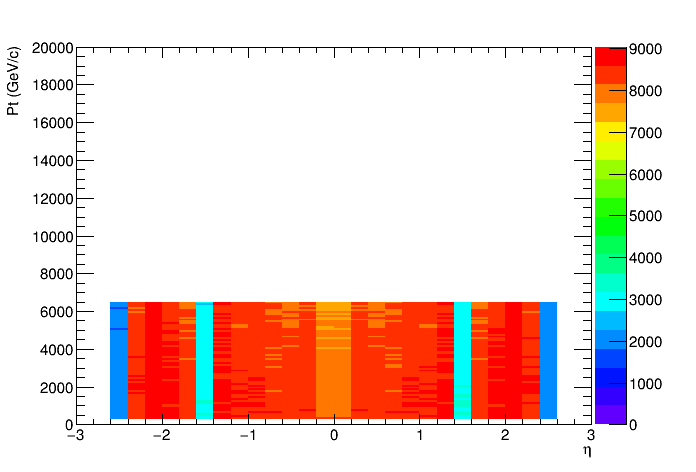
\includegraphics[width=0.45\textwidth]{chapters/Zprime/Saturation/images/FlatPt/Sample_variables/Ptmc_eta.png} &
      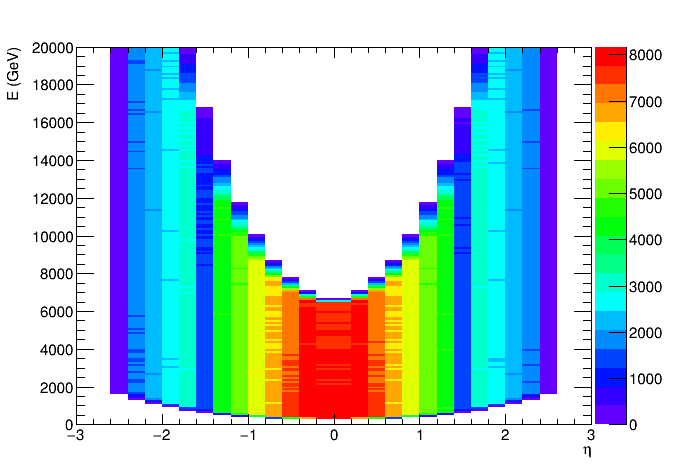
\includegraphics[width=0.45\textwidth]{chapters/Zprime/Saturation/images/FlatPt/Sample_variables/Emc_eta.png} \\
      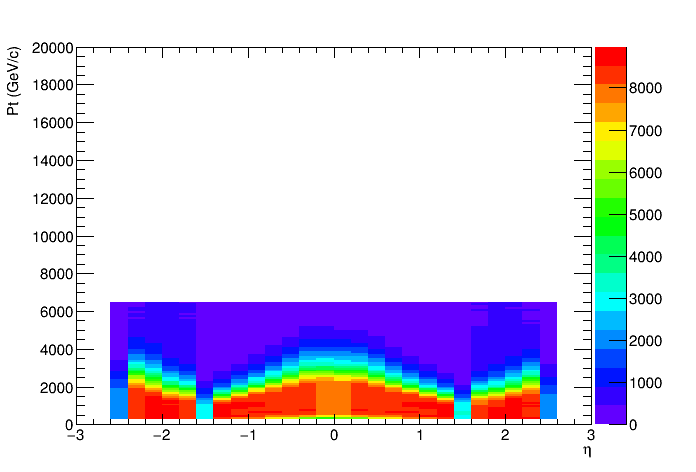
\includegraphics[width=0.45\textwidth]{chapters/Zprime/Saturation/images/FlatPt/Sample_variables/Ptmc_eta_nos.png} &
      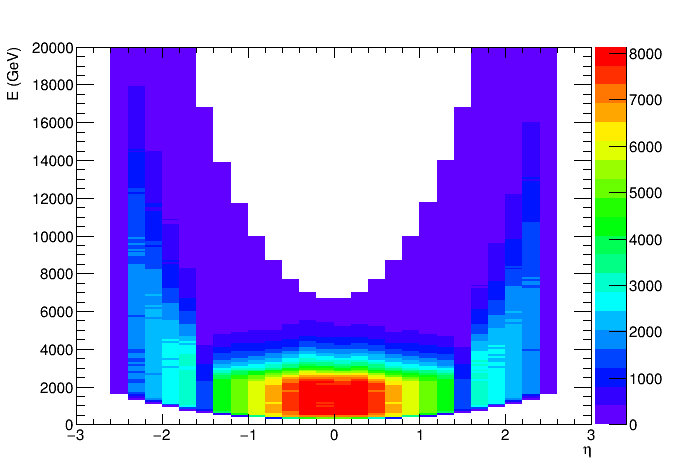
\includegraphics[width=0.45\textwidth]{chapters/Zprime/Saturation/images/FlatPt/Sample_variables/Emc_eta_nos.png} \\
      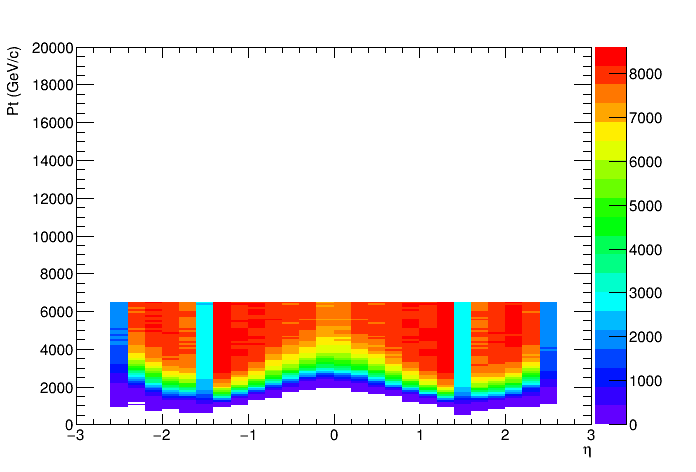
\includegraphics[width=0.45\textwidth]{chapters/Zprime/Saturation/images/FlatPt/Sample_variables/Ptmc_eta_s.png} &
      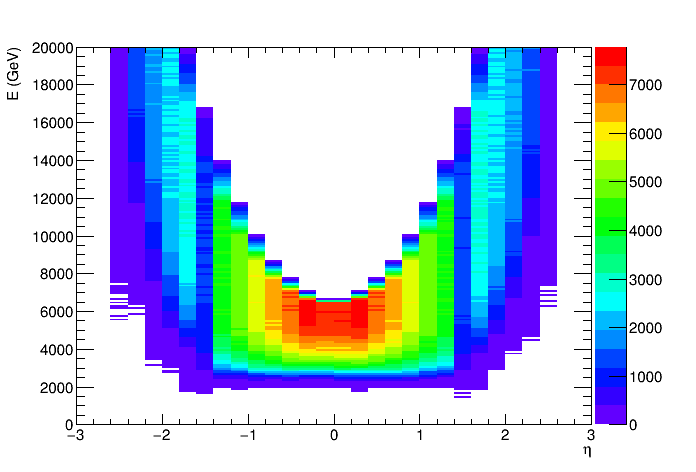
\includegraphics[width=0.45\textwidth]{chapters/Zprime/Saturation/images/FlatPt/Sample_variables/Emc_eta_s.png} \\
    \end{tabular}
    \caption{The distributions of $P_{T}$ for generated electrons versus $\eta$ (left) and energy of generated electrons versus $\eta$ (right) for all electrons (top), unsaturated electrons (middle) and saturated electrons (bottom).}
    \label{fig:Ptmc_Emc_eta}
  \end{center}
\end{figure}


\begin{figure}[bh]
  \begin{center}
    \begin{tabular}{cc}
      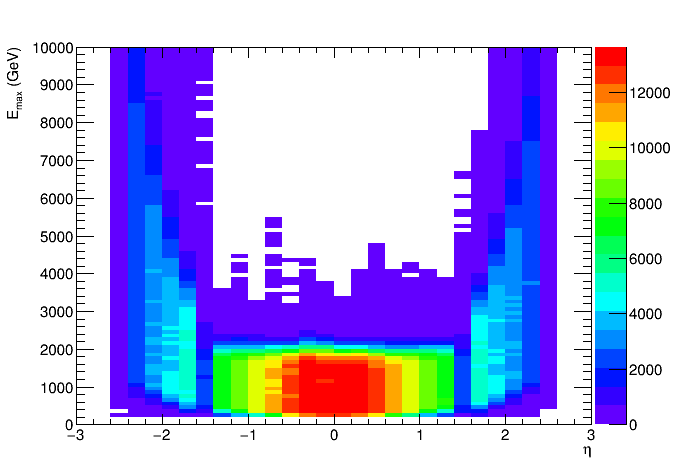
\includegraphics[width=0.45\textwidth]{chapters/Zprime/Saturation/images/FlatPt/Sample_variables/Emax_eta_nos.png} &
      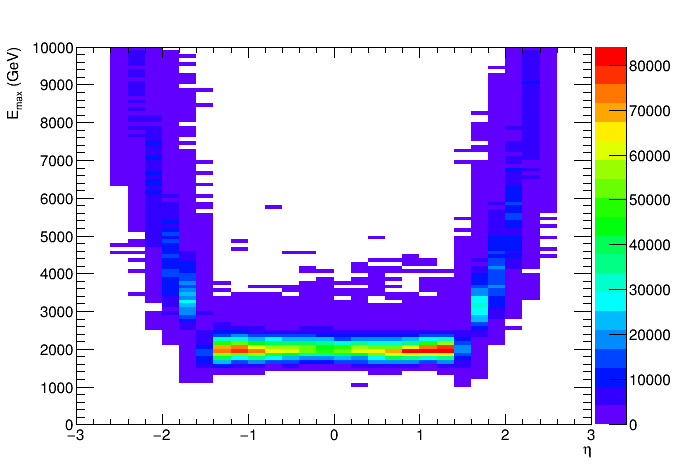
\includegraphics[width=0.45\textwidth]{chapters/Zprime/Saturation/images/FlatPt/Sample_variables/Emax_eta_s.png} \\
    \end{tabular}
    \caption{The distributions of $E_{max}$ versus $\eta$ for unsaturated electrons (left) and saturated electrons (right).}
    \label{fig:Emax_eta}
  \end{center}
\end{figure}


\begin{figure}[bh]
  \begin{center}
    \begin{tabular}{cc}
      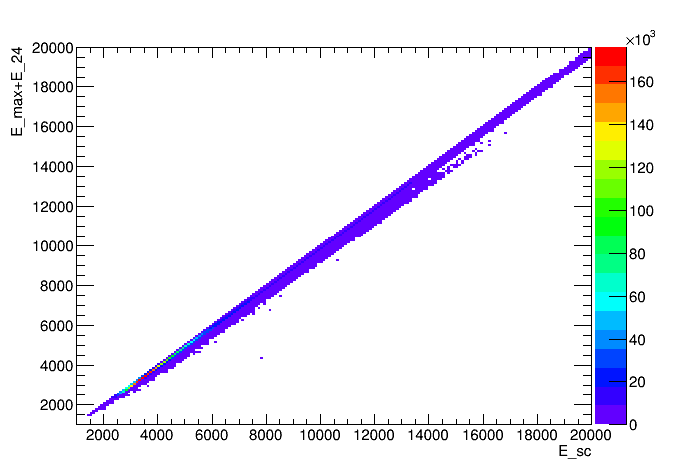
\includegraphics[width=0.45\textwidth]{chapters/Zprime/Saturation/images/FlatPt/Sample_variables/Esc_EmaxE24.png}
    \end{tabular}
    \caption{The distribution of $E_{max}~ + ~E_{24}$ versus $E_{sc}$ for saturated electrons.}
    \label{fig:EmaxE24_Esc}
  \end{center}
\end{figure}

\begin{figure}[bh]
  \begin{center}
    \begin{tabular}{cc}
      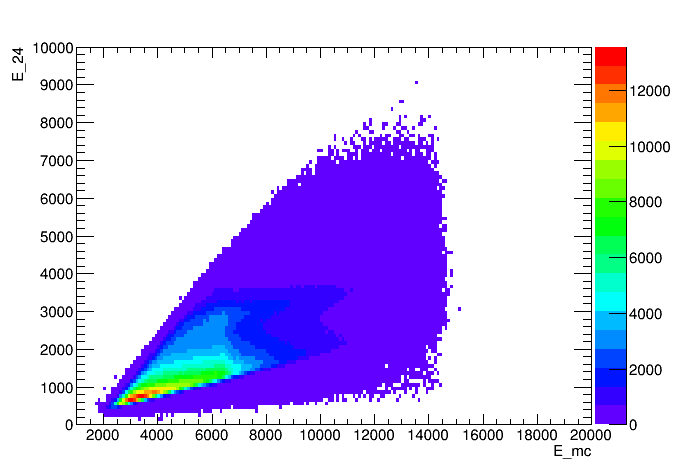
\includegraphics[width=0.45\textwidth]{chapters/Zprime/Saturation/images/FlatPt/Sample_variables/Emc_E24_Barrel.png} &
      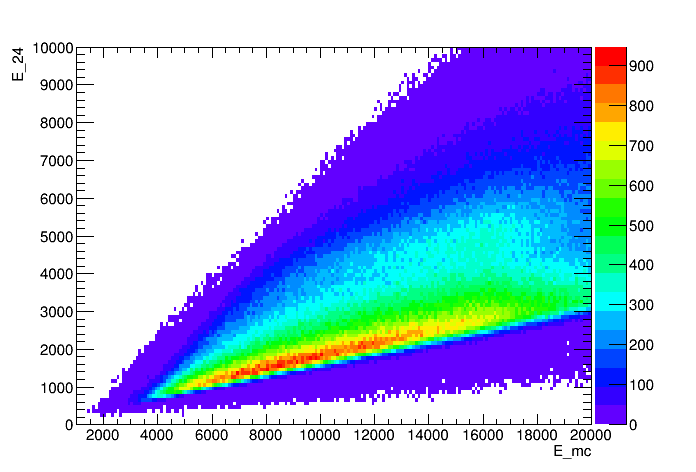
\includegraphics[width=0.45\textwidth]{chapters/Zprime/Saturation/images/FlatPt/Sample_variables/Emc_E24_Endcap.png} \\
      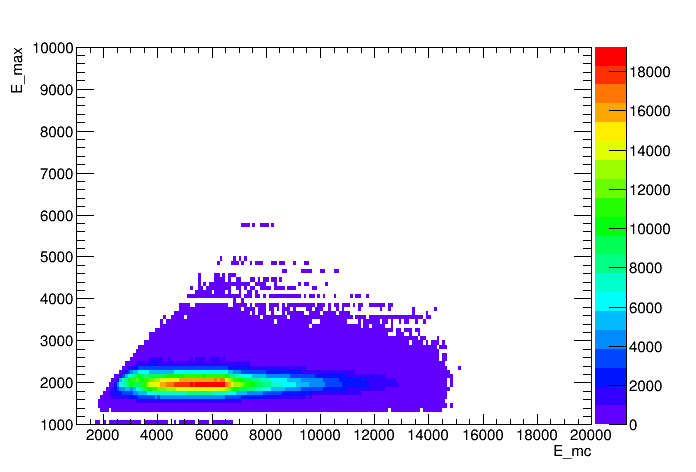
\includegraphics[width=0.45\textwidth]{chapters/Zprime/Saturation/images/FlatPt/Sample_variables/Emc_Emax_Barrel.png} &
      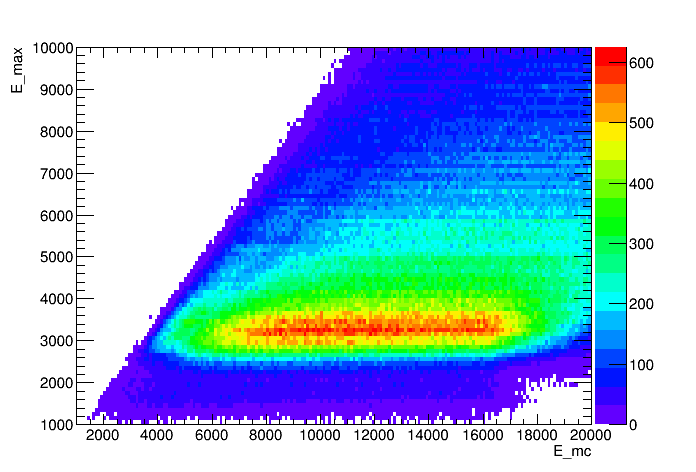
\includegraphics[width=0.45\textwidth]{chapters/Zprime/Saturation/images/FlatPt/Sample_variables/Emc_Emax_Endcap.png} \\
      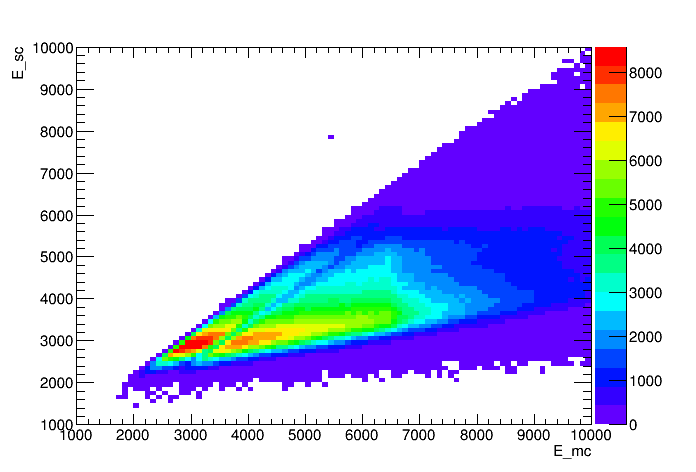
\includegraphics[width=0.45\textwidth]{chapters/Zprime/Saturation/images/FlatPt/Sample_variables/Emc_Esc_Barrel.png} &
      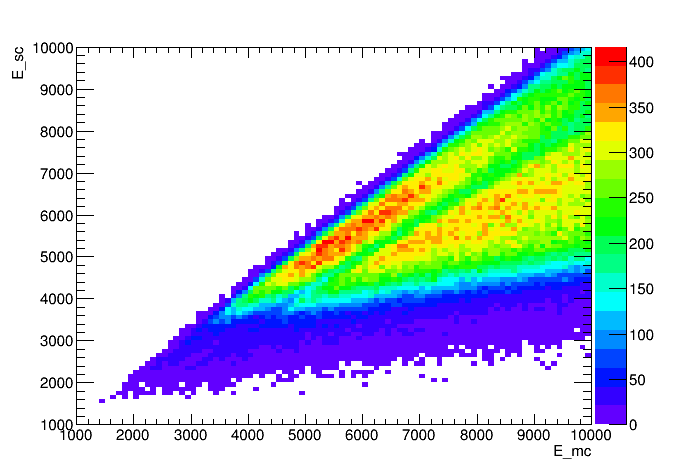
\includegraphics[width=0.45\textwidth]{chapters/Zprime/Saturation/images/FlatPt/Sample_variables/Emc_Esc_Endcap.png} \\
    \end{tabular}
    \caption{The distributions of $E_{24}$ versus $E_{mc}$ (top), $E_{max}$ versus $E_{mc}$ (middle) and $E_{sc}$ versus $E_{mc}$ (bottom) for saturated electrons for barrel (left) and endcap (right).}
    \label{fig:Esc_Emc}
  \end{center}
\end{figure}

\begin{figure}[bh]
  \begin{center}
    \begin{tabular}{cc}
      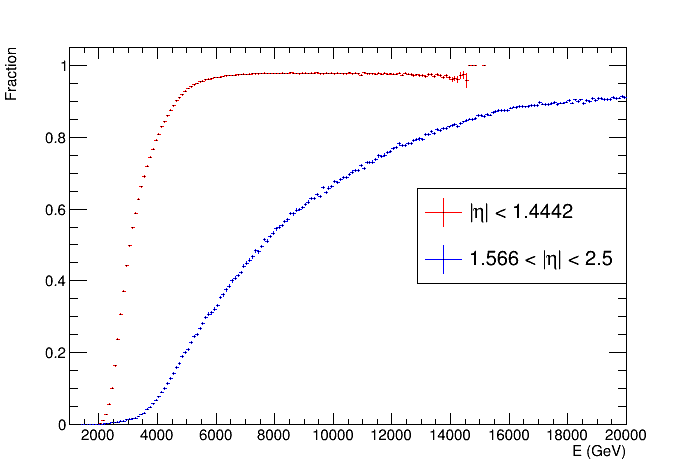
\includegraphics[width=0.9\textwidth]{chapters/Zprime/Saturation/images/FlatPt/Sample_variables/Barrel_Endcap_fraction.png}
    \end{tabular}
    \caption{The saturated fraction versus true (or mc) energy of electron for barrel (red points) and endcap (blue points).}
    \label{fig:S_Fraction}
  \end{center}
\end{figure}

\begin{figure}[bh]
  \begin{center}
    \begin{tabular}{cc}
      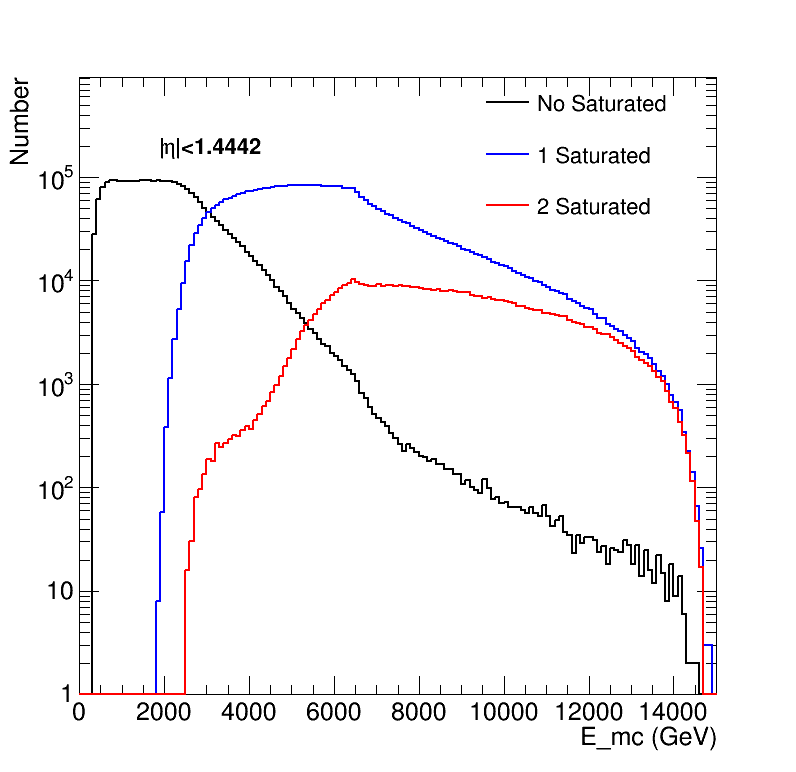
\includegraphics[width=0.45\textwidth]{chapters/Zprime/Saturation/images/FlatPt/Sample_variables/N_s_vs_Emc_Barrel.png} &
      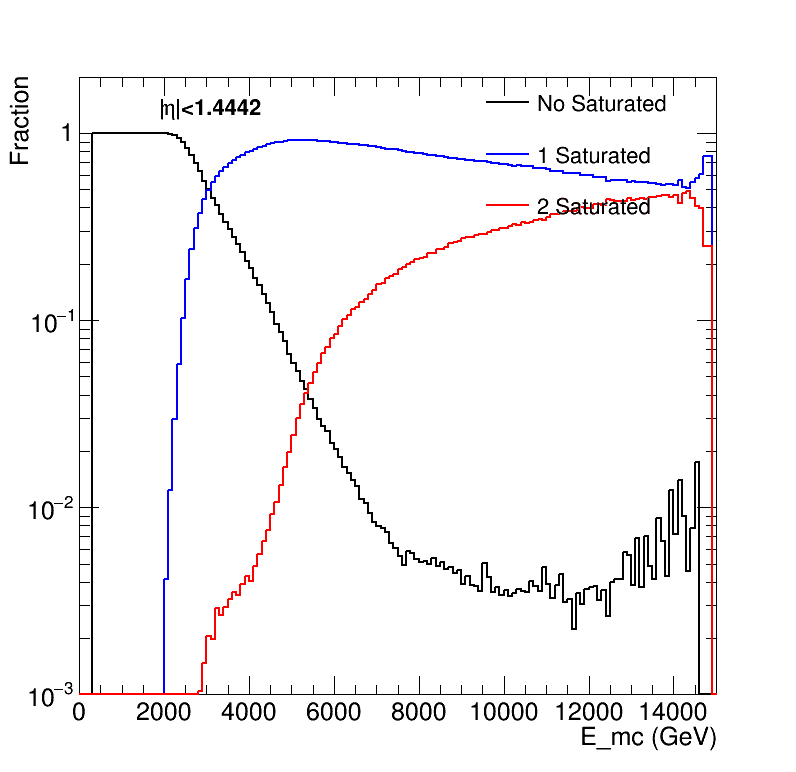
\includegraphics[width=0.45\textwidth]{chapters/Zprime/Saturation/images/FlatPt/Sample_variables/N_s_vs_Emc_fraBarrel.png} \\
      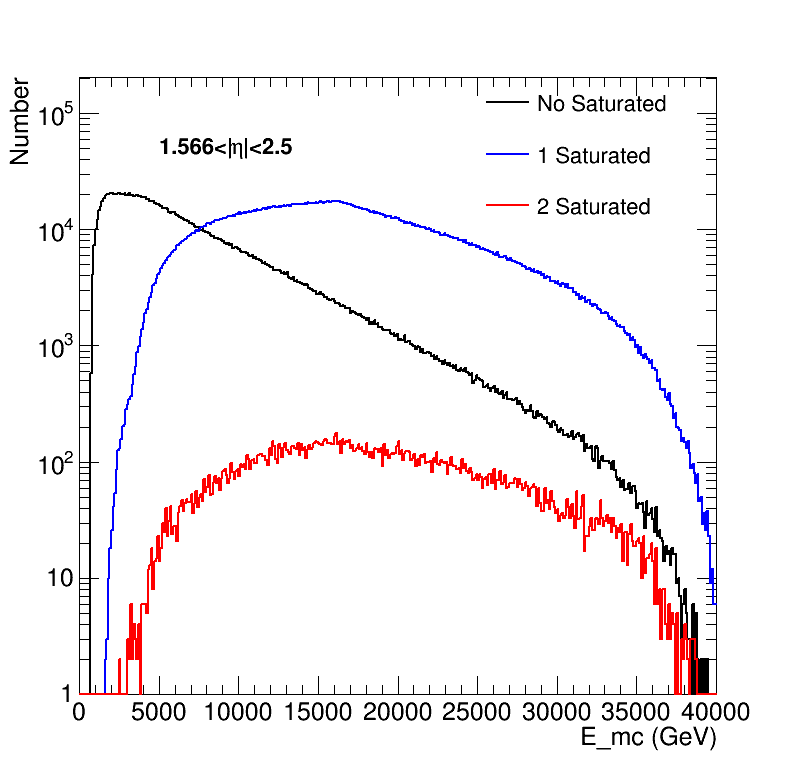
\includegraphics[width=0.45\textwidth]{chapters/Zprime/Saturation/images/FlatPt/Sample_variables/N_s_vs_Emc_Endcap.png} &
      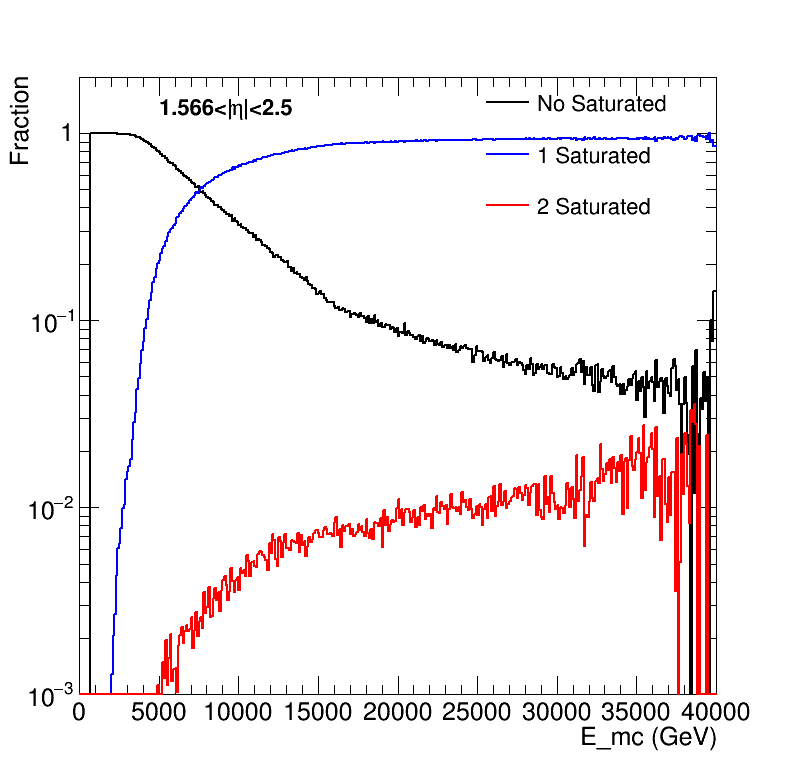
\includegraphics[width=0.45\textwidth]{chapters/Zprime/Saturation/images/FlatPt/Sample_variables/N_s_vs_Emc_fraEndcap.png} \\
    \end{tabular}
    \caption{The number of saturated crystals in $3\times3$ matrix with seed crystal in the center for different mc energy (left) and the fraction of number of saturated crystals in $3\times3$ matrix with seed crystal in the center for different mc energy (right) for barrel (top) and endcap (bottom).}
    \label{fig:N_S_Emc}
  \end{center}
\end{figure}

\subsubsection{Result}

The distribution of $(reco E - true E)/true E$ are shown in Figure \ref{fig:result_B_E} and one can see the energy of saturated electron from MVA is very close to true (or mc) energy. A fit to the MVA result using double-side CB is performed, the peak position and the standard deviation of the Gaussian core of the distributions are estimated through the fitted values of mean and sigma, respectively. The $'effective'$ standard deviation $\sigma_{eff}$, defined as half of the smallest interval around the peak position containing 68.3\% of the events, is used to assess the resolution, while taking into account possible non-Gaussian tails. We also checked the result by using MLP method which gives worse resolution shown in Figure \ref{fig:MLP_B_E} in section \ref{MLP_check}, therefore our basic method is BDTG method. Then we check the results for different $\eta$ which are shown in Figure \ref{fig:result_B123} and \ref{fig:result_E12}. From figures \ref{fig:result_B123} and \ref{fig:result_E12} we know the MVA works well for different $\eta$. Besides we check the MVA regressive results for different true energy of saturated electron which are shown in Figure \ref{fig:result_energy}. From Figure \ref{fig:result_energy} we see for barrel the results are stable for different energy, while for endcap the results are not very well in low energy, because for low electron energy the possibility of crystal to be saturated in endcap is very small and the training statistics for low energy and saturated electron is very less which can be seen in the bottom right plot of Figure \ref{fig:Ptmc_Emc_eta}.

\begin{figure}[bh]
  \begin{center}
    \begin{tabular}{cc}
      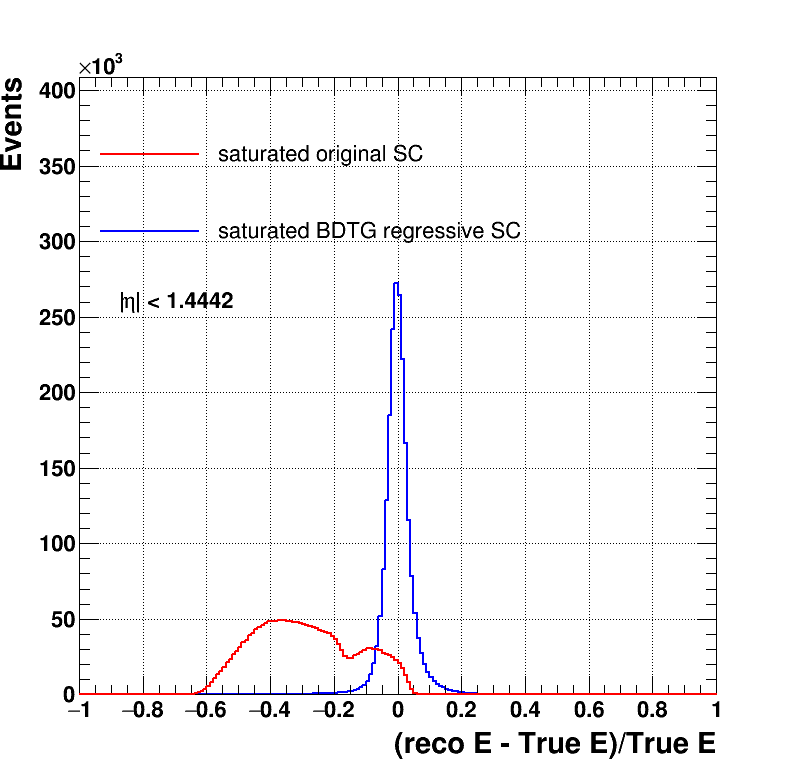
\includegraphics[width=0.45\textwidth]{chapters/Zprime/Saturation/images/FlatPt/Result/Barrel_Endcap/compare_BDTG_Barrel_Endcap_enSC_B_s.png} &
      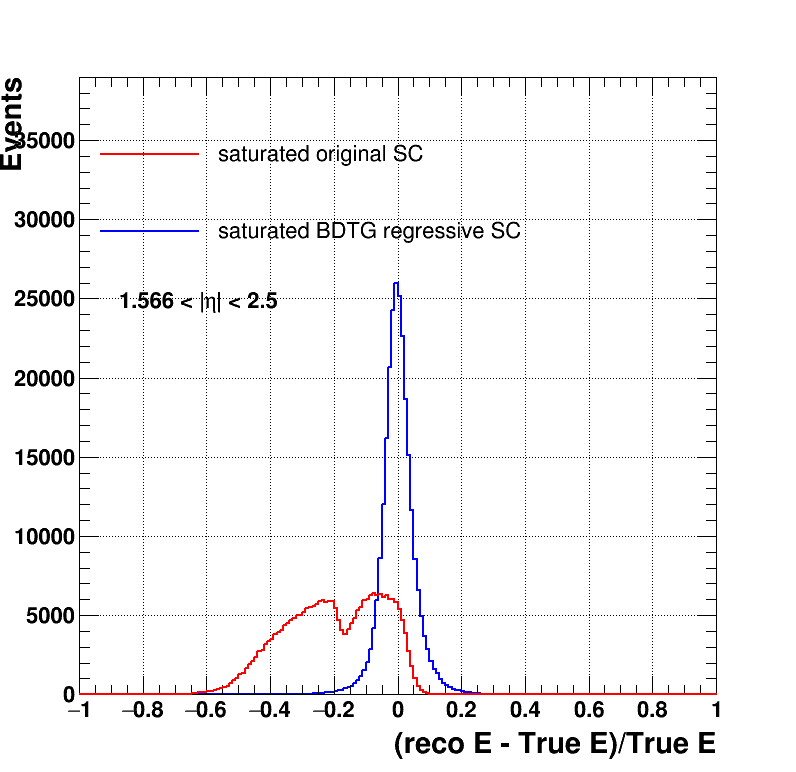
\includegraphics[width=0.45\textwidth]{chapters/Zprime/Saturation/images/FlatPt/Result/Barrel_Endcap/compare_BDTG_Barrel_Endcap_enSC_E_s.png} \\
      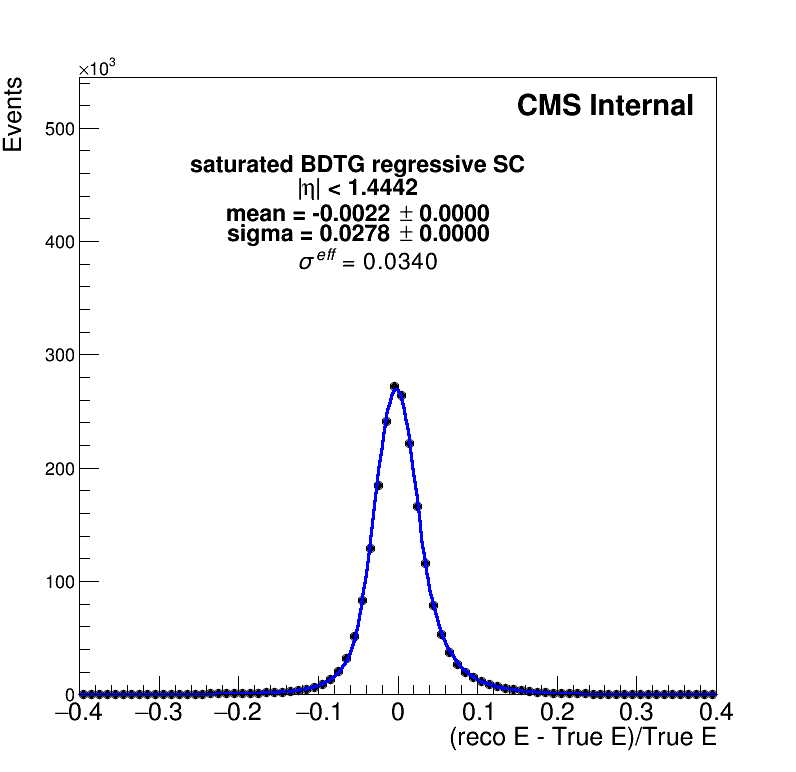
\includegraphics[width=0.45\textwidth]{chapters/Zprime/Saturation/images/FlatPt/Result/Barrel_Endcap/fit_BDTG_Barrel_Endcap_B_reg_s.png} &
      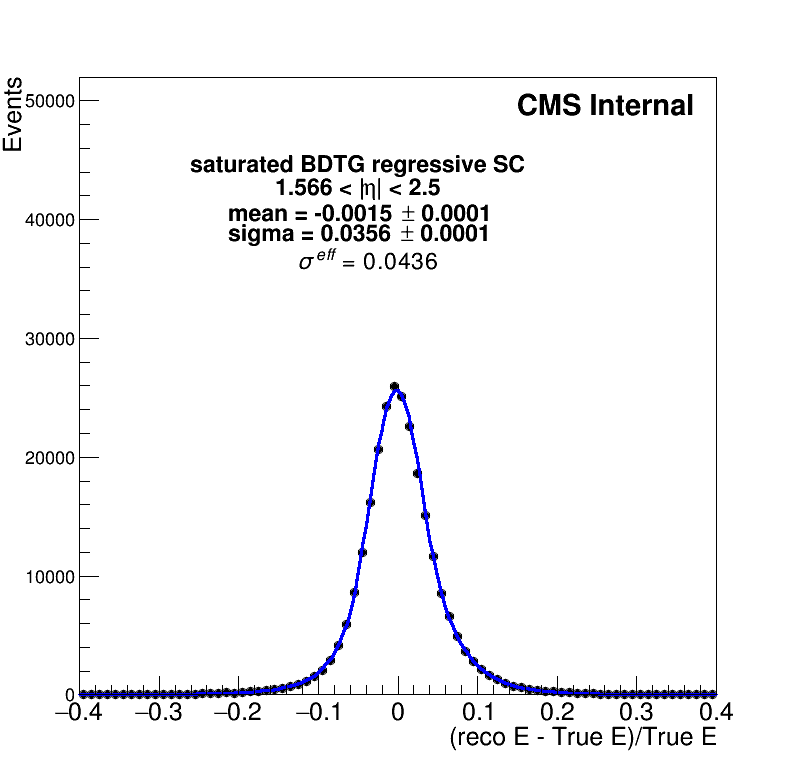
\includegraphics[width=0.45\textwidth]{chapters/Zprime/Saturation/images/FlatPt/Result/Barrel_Endcap/fit_BDTG_Barrel_Endcap_E_reg_s.png}
    \end{tabular}
    \caption{ The top plots are the distribution of supercluster energy minus ture energy divided by true energy for saturated electron for barrel (left) and endcap (right), the red histogram is for reconstructed supercluster enery, the blue histogram is for MVA regressive energy. The bottom plots are the fit of the blue histogram for barrel (left) and endcap (right).}
    \label{fig:result_B_E}
  \end{center}
\end{figure}



\begin{figure}[bh]
  \begin{center}
    \begin{tabular}{cc}
      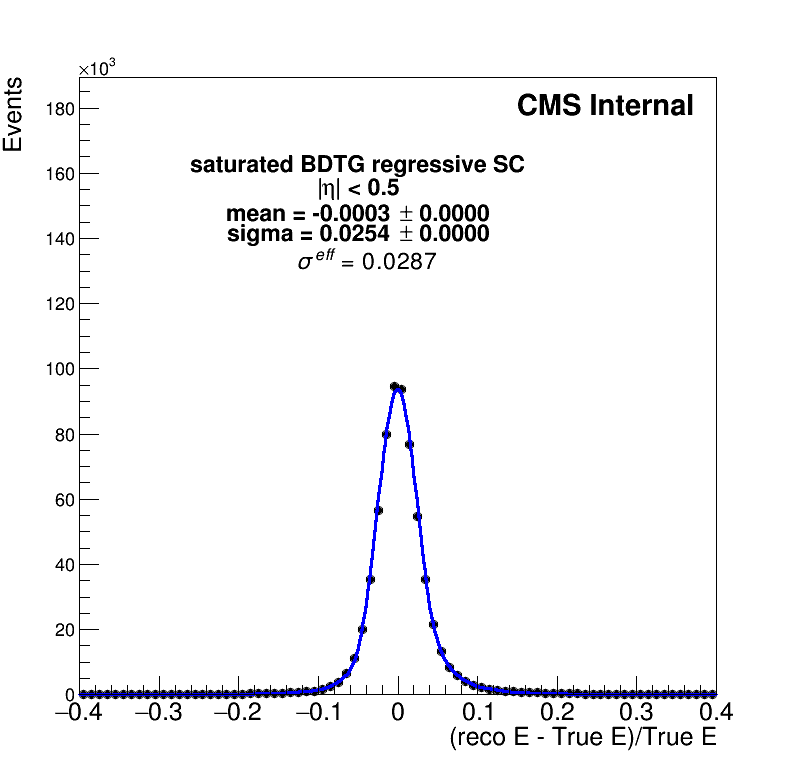
\includegraphics[width=0.45\textwidth]{chapters/Zprime/Saturation/images/FlatPt/Result/Barrel123_Endcap12/fit_BDTG_Barrel123_Endcap12_eta1_reg_s.png} &
      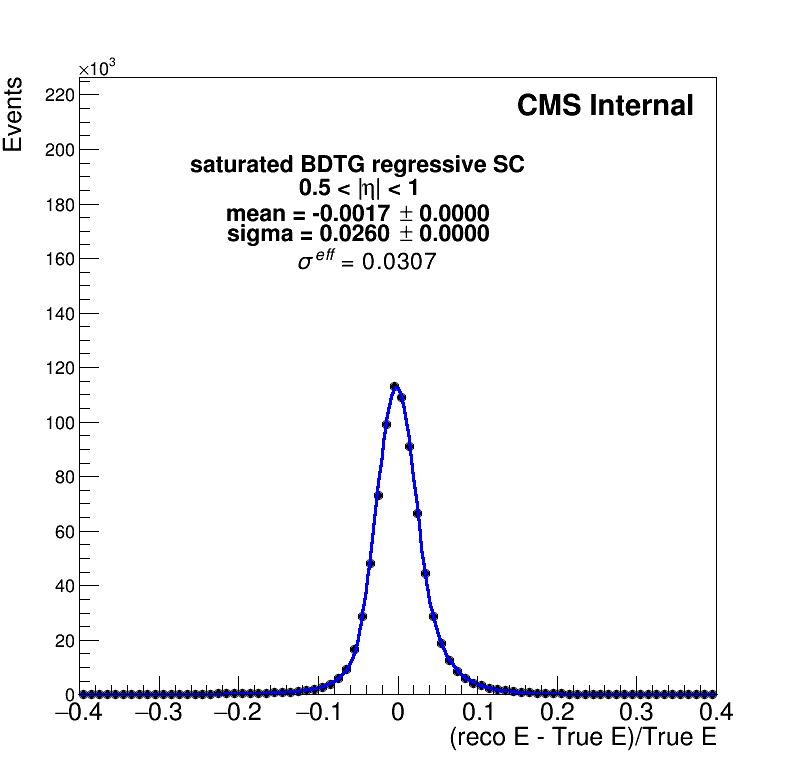
\includegraphics[width=0.45\textwidth]{chapters/Zprime/Saturation/images/FlatPt/Result/Barrel123_Endcap12/fit_BDTG_Barrel123_Endcap12_eta2_reg_s.png} \\
      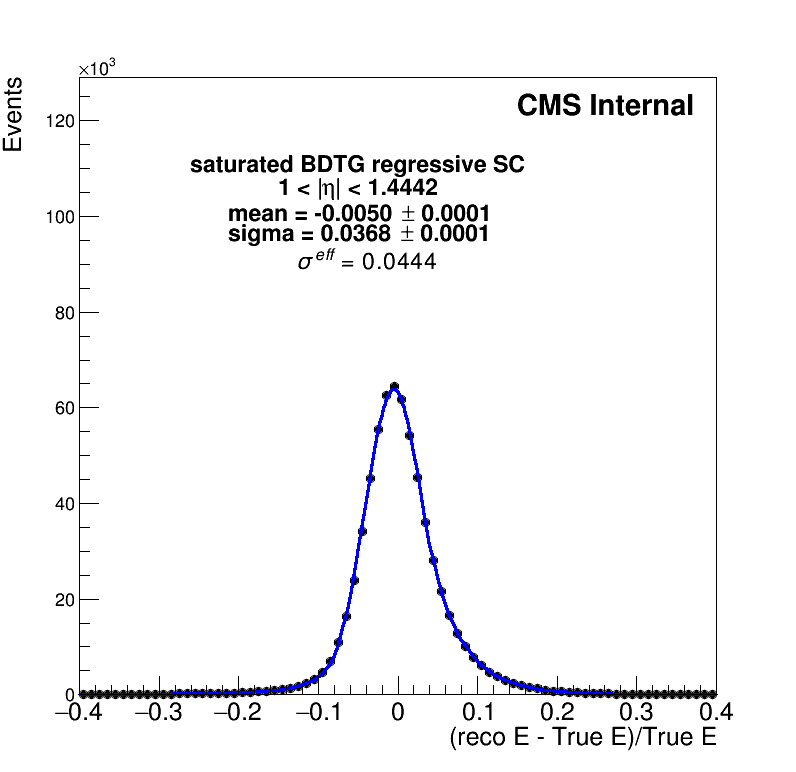
\includegraphics[width=0.45\textwidth]{chapters/Zprime/Saturation/images/FlatPt/Result/Barrel123_Endcap12/fit_BDTG_Barrel123_Endcap12_eta3_reg_s.png} &
    \end{tabular}
    \caption{ The distributions of MVA regressive energy minus ture energy divided by true energy for saturated electrons in barrel for different $\eta$ ranges.}
    \label{fig:result_B123}
  \end{center}
\end{figure}


\begin{figure}[bh]
  \begin{center}
    \begin{tabular}{cc}
      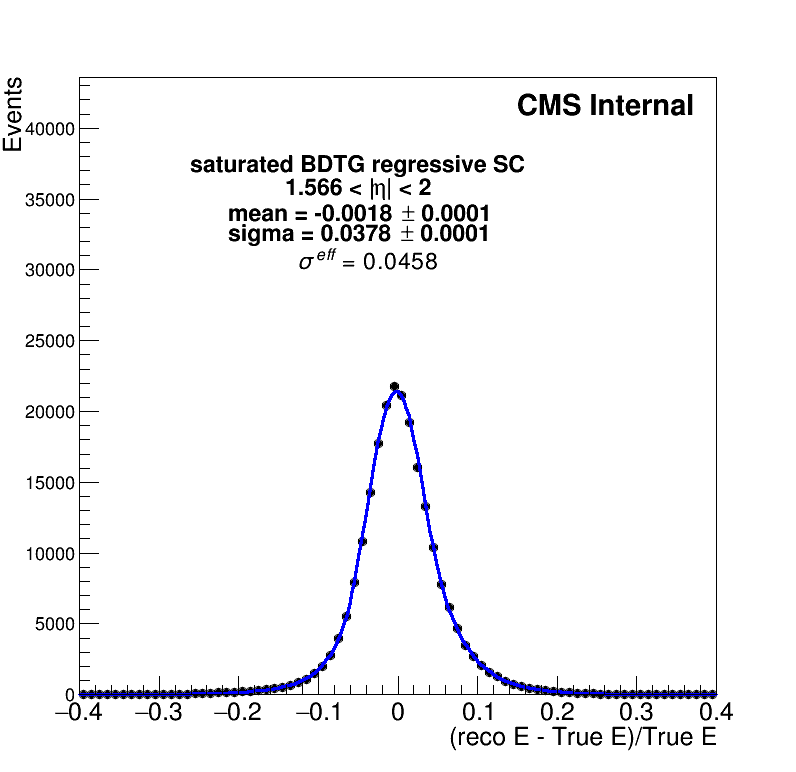
\includegraphics[width=0.45\textwidth]{chapters/Zprime/Saturation/images/FlatPt/Result/Barrel123_Endcap12/fit_BDTG_Barrel123_Endcap12_Eeta1_reg_s.png} &
      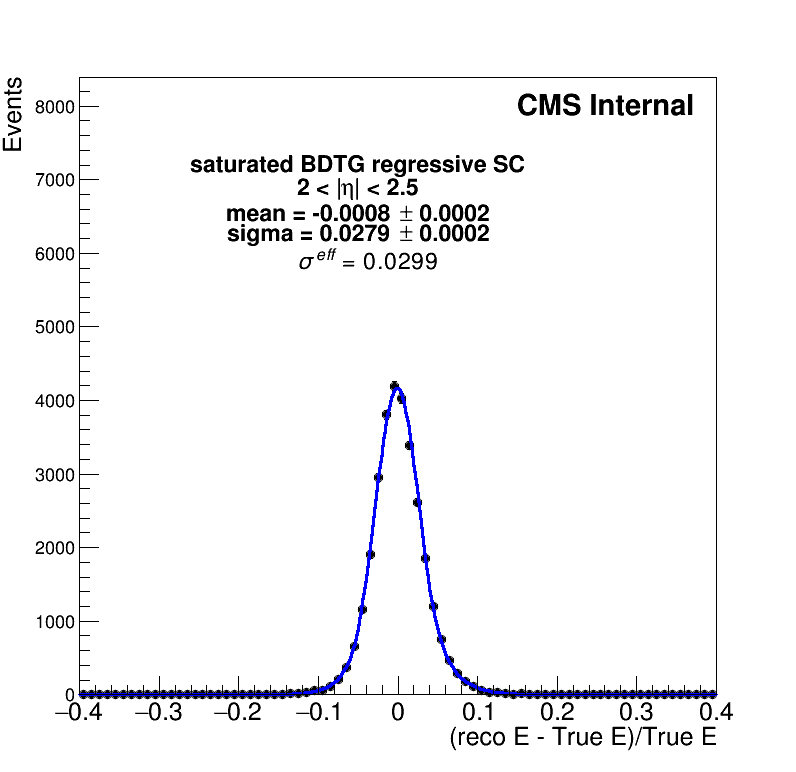
\includegraphics[width=0.45\textwidth]{chapters/Zprime/Saturation/images/FlatPt/Result/Barrel123_Endcap12/fit_BDTG_Barrel123_Endcap12_Eeta2_reg_s.png} \\
    \end{tabular}
    \caption{ The distributions of MVA regressive energy minus ture energy divided by true energy for saturated electron in endcap for different $\eta$ ranges.}
    \label{fig:result_E12}
  \end{center}
\end{figure}


\begin{figure}[bh]
  \begin{center}
    \begin{tabular}{cc}
      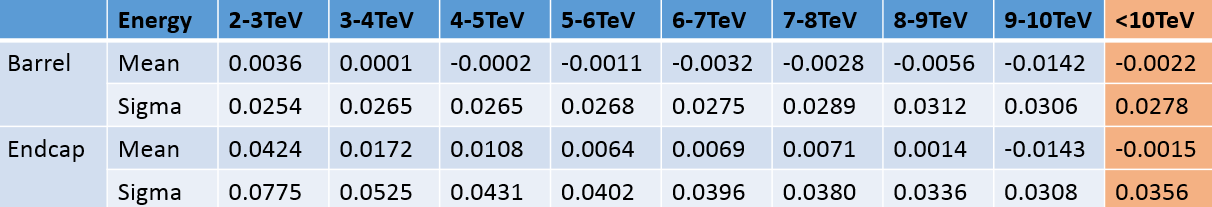
\includegraphics[width=0.9\textwidth]{chapters/Zprime/Saturation/images/FlatPt/Result/different_energy.png}
    \end{tabular}
    \caption{ The fit results for the distributions of MVA regressive energy minus ture energy divided by true energy for saturated electron for different true energy in barrel and endcap.}
    \label{fig:result_energy}
  \end{center}
\end{figure}

\subsubsection{Check the result in ZToEE samples}

Here we check the MVA result using ZToEE powheg sample with $M_{Z}$ great than 4500 GeV samples. The results are shown in figures \ref{fig:ZToEE_4500_6000_B_E} and \ref{fig:ZToEE_6000_Inf_B_E}. The result looks good.

\begin{figure}[bh]
  \begin{center}
    \begin{tabular}{cc}
      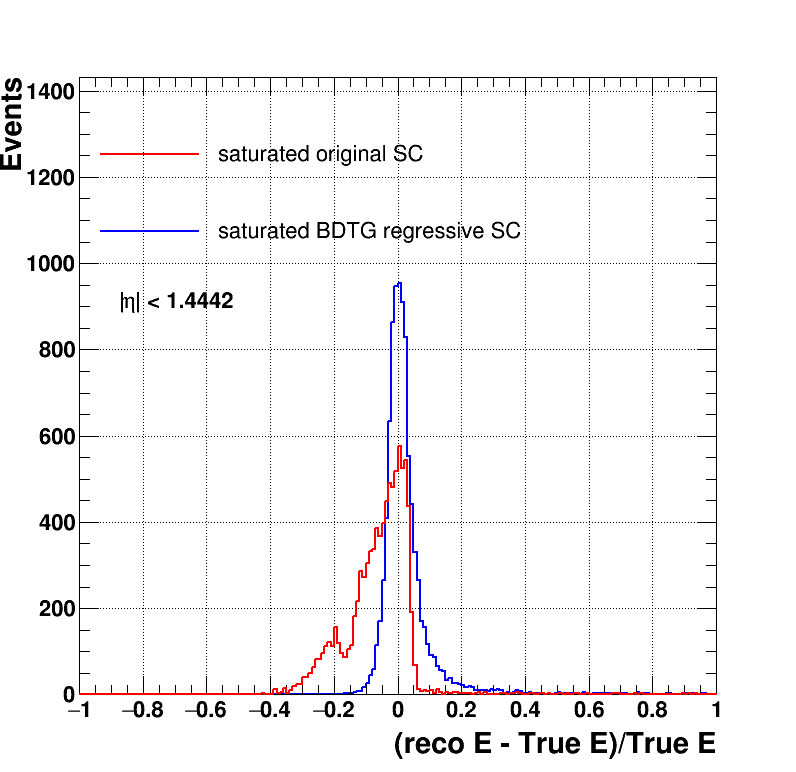
\includegraphics[width=0.45\textwidth]{chapters/Zprime/Saturation/images/FlatPt/ZToEE_check/4500_6000/compare_BDTG_Barrel_Endcap_enSC_B_s.png} &
      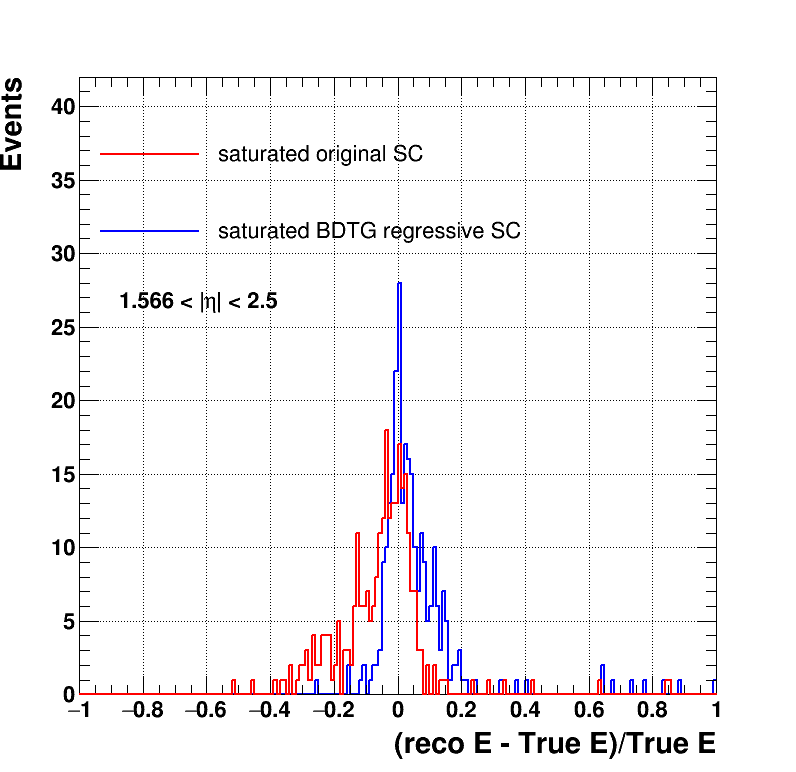
\includegraphics[width=0.45\textwidth]{chapters/Zprime/Saturation/images/FlatPt/ZToEE_check/4500_6000/compare_BDTG_Barrel_Endcap_enSC_E_s.png} \\
      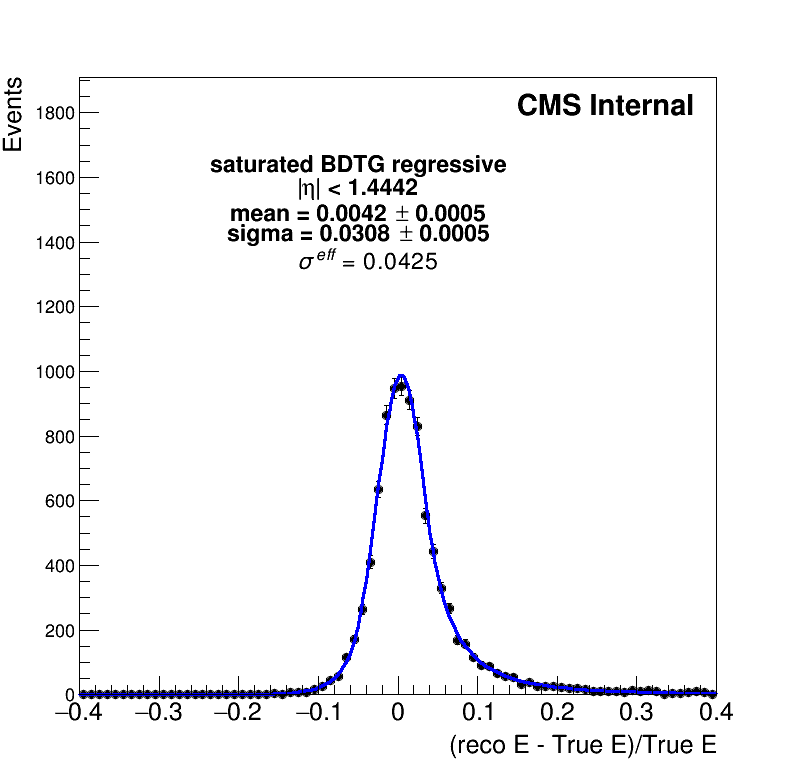
\includegraphics[width=0.45\textwidth]{chapters/Zprime/Saturation/images/FlatPt/ZToEE_check/4500_6000/fit_BDTG_Barrel_Endcap_B_reg_s.png} &
      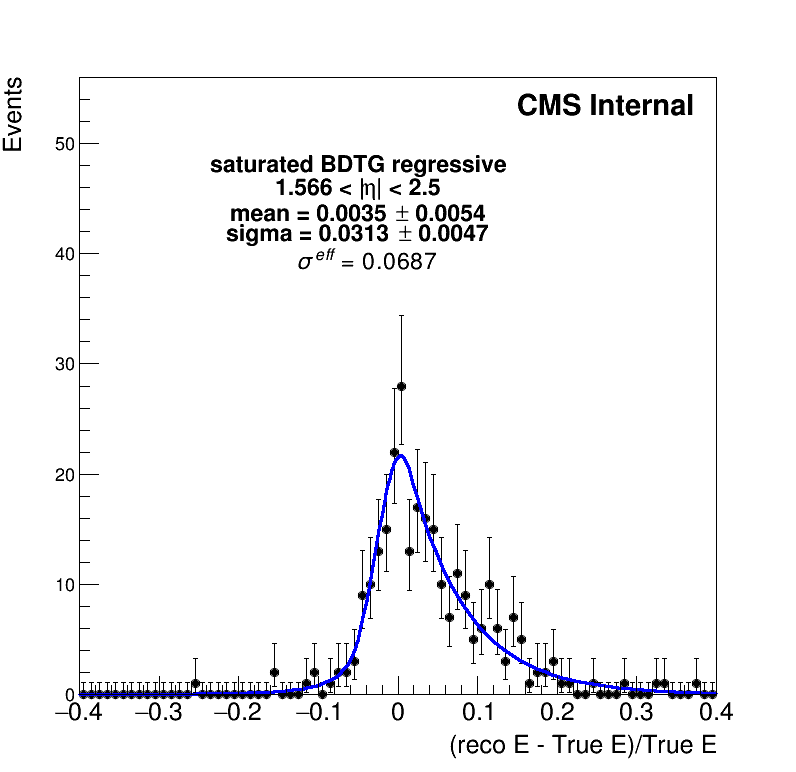
\includegraphics[width=0.45\textwidth]{chapters/Zprime/Saturation/images/FlatPt/ZToEE_check/4500_6000/fit_BDTG_Barrel_Endcap_E_reg_s.png}
    \end{tabular}
    \caption{ The top plots are the distribution of supercluster energy minus ture energy divided by true energy for saturated electron for barrel (left) and endcap (right) for ZToEE\_4500\_6000 sample, the red histogram is for reconstructed supercluster enery, the blue histogram is for MVA regressive energy. The bottom plots are the fit of the blue histogram for barrel (left) and endcap (right).}
    \label{fig:ZToEE_4500_6000_B_E}
  \end{center}
\end{figure}


\begin{figure}[bh]
  \begin{center}
    \begin{tabular}{cc}
      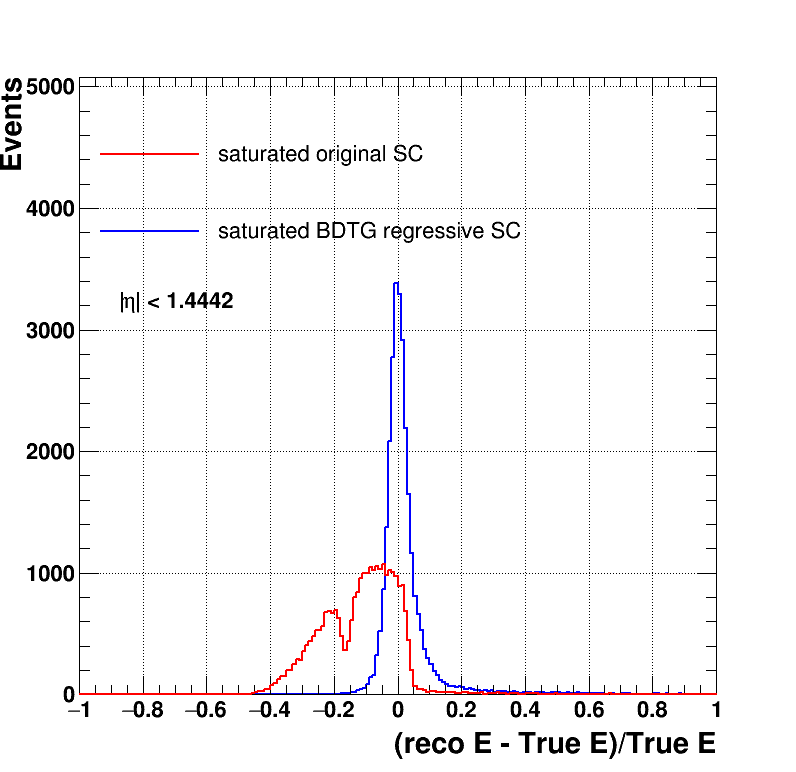
\includegraphics[width=0.45\textwidth]{chapters/Zprime/Saturation/images/FlatPt/ZToEE_check/6000_Inf/compare_BDTG_Barrel_Endcap_enSC_B_s.png} &
      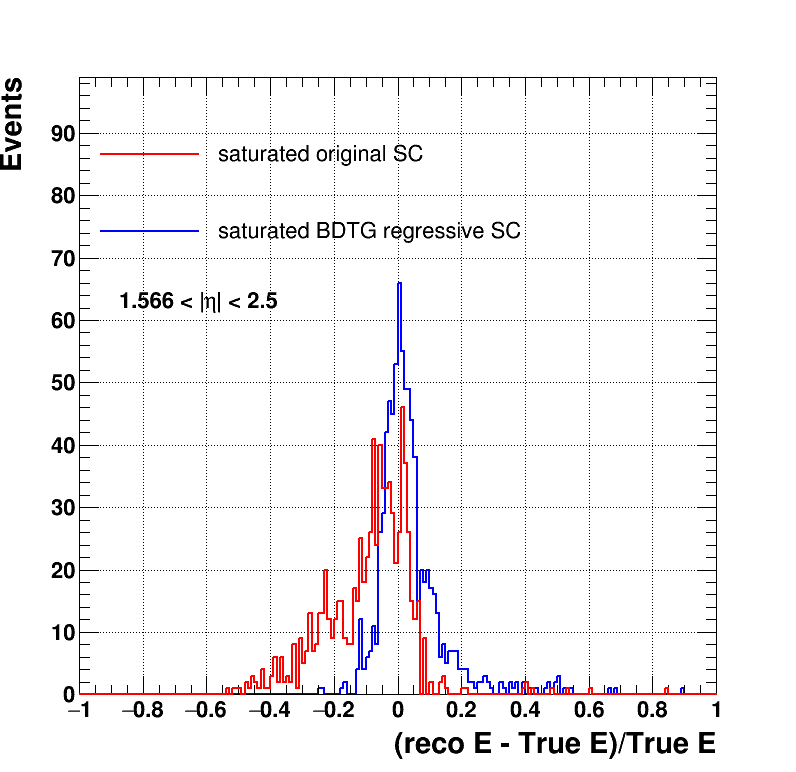
\includegraphics[width=0.45\textwidth]{chapters/Zprime/Saturation/images/FlatPt/ZToEE_check/6000_Inf/compare_BDTG_Barrel_Endcap_enSC_E_s.png} \\
      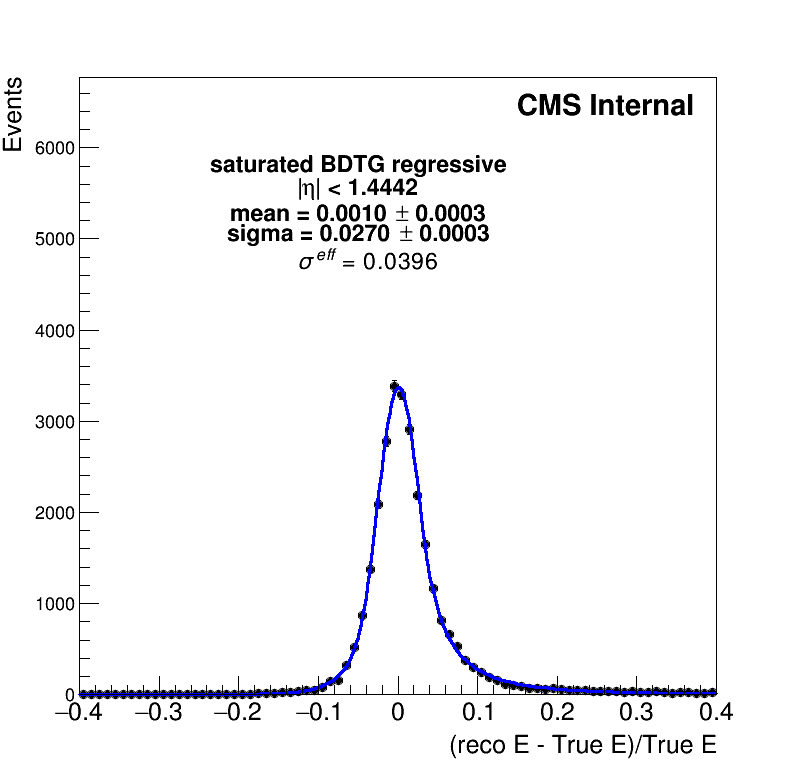
\includegraphics[width=0.45\textwidth]{chapters/Zprime/Saturation/images/FlatPt/ZToEE_check/6000_Inf/fit_BDTG_Barrel_Endcap_B_reg_s.png} &
      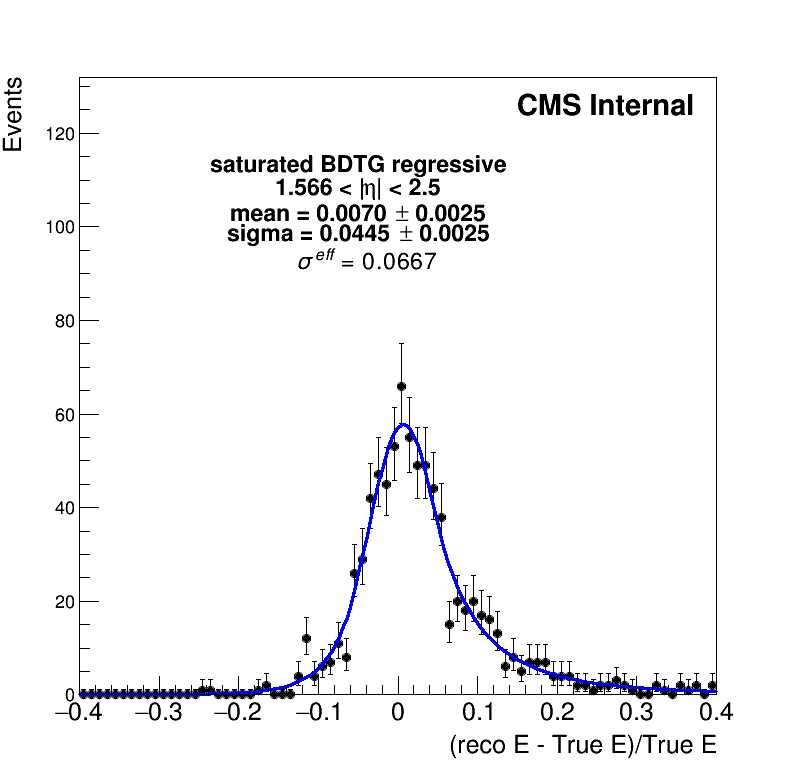
\includegraphics[width=0.45\textwidth]{chapters/Zprime/Saturation/images/FlatPt/ZToEE_check/6000_Inf/fit_BDTG_Barrel_Endcap_E_reg_s.png}
    \end{tabular}
    \caption{ The top plots are the distribution of supercluster energy minus ture energy divided by true energy for saturated electron for barrel (left) and endcap (right) for ZToEE$\_$6000$\_$Inf sample, the red histogram is for reconstructed supercluster enery, the blue histogram is for MVA regressive energy. The bottom plots are the fit of the blue histogram for barrel (left) and endcap (right).}
    \label{fig:ZToEE_6000_Inf_B_E}
  \end{center}
\end{figure}


\subsubsection{Apply to data}

Using DoubleEG dataset from 2016 in \ref{tab:Zprime-data-samples}, we find three events in which there are and only one saturated HEEP (High Energy Electron Pairs) electron. The energy of SC and MVA regressived energy are shown in Table  \ref{tab:detail}. The events displays are shown in Figure \ref{fig:event_display}.

\begin{table}[!h]
  \begin{center}
\smallskip\noindent
\resizebox{\linewidth}{!}{%
    \begin{tabular}{lllll}
      \hline
                    & event number & $\eta$    & SC energy (GeV)  & Regressived energy (GeV)  \\
      \hline
      electron1     & 1076867675   & 1.21759 & 2370.34          & 2279.53                   \\
      electron2     & 897834686    & 1.56931 & 2954.7           & 3167.63                   \\
      electron3     & 400840829    & 1.1476  & 2048.81          & 3151.99                   \\
      \hline
    \end{tabular}}
    \caption{Detail of saturated HEEP electrons.}
    \label{tab:detail}
  \end{center}
\end{table}

\begin{figure}[bh]
  \begin{center}
    \begin{tabular}{cc}
      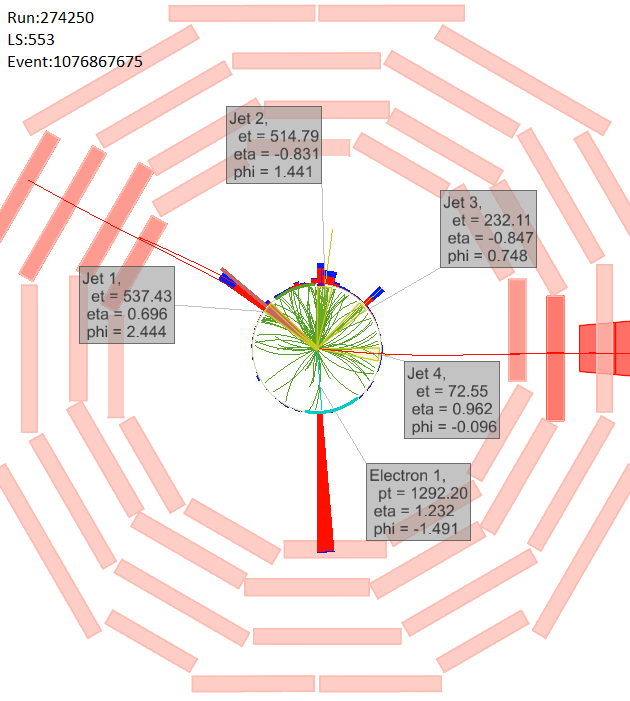
\includegraphics[width=0.45\textwidth]{chapters/Zprime/Saturation/images/FlatPt/cmsShow/274250_1076867675_553_RhoPhi.png} &
      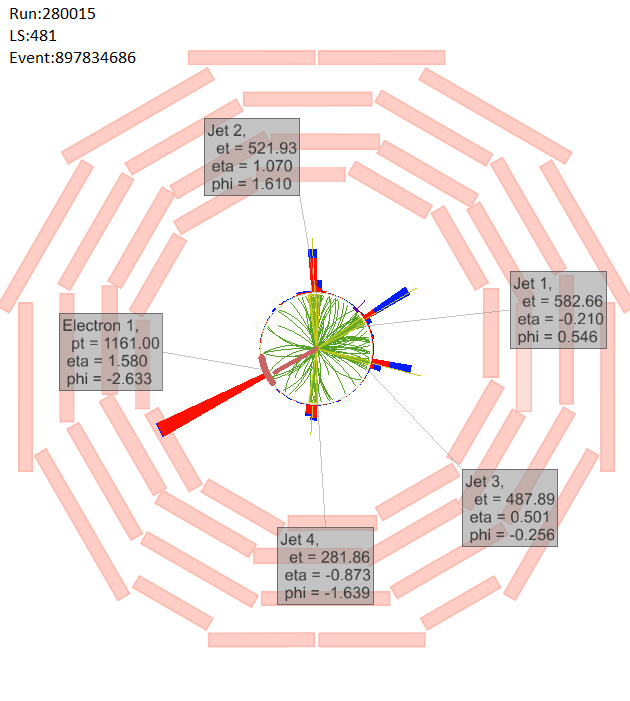
\includegraphics[width=0.45\textwidth]{chapters/Zprime/Saturation/images/FlatPt/cmsShow/280015_897834686_481_RhoPhi.png} \\
      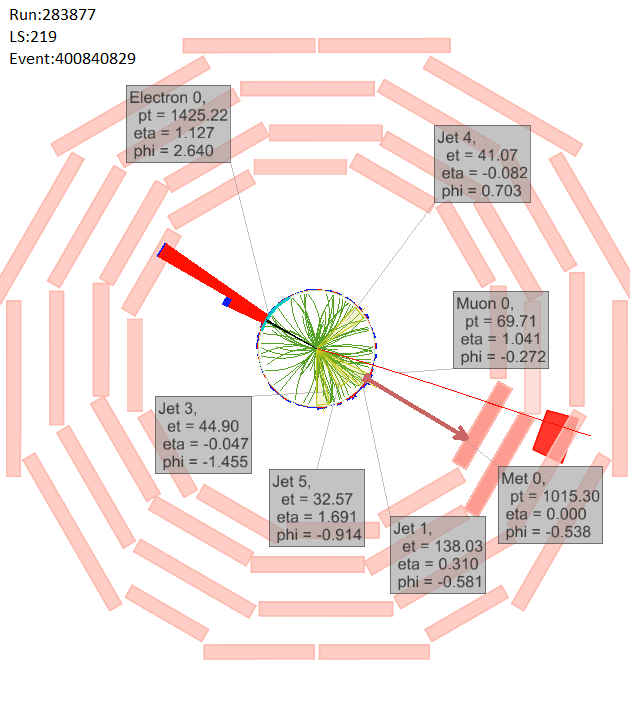
\includegraphics[width=0.45\textwidth]{chapters/Zprime/Saturation/images/FlatPt/cmsShow/283877_400840829_219_RhoPhi.png}
    \end{tabular}
    \caption{ The events displays of saturated HEEP electrons in data for $\rho\phi$ visual angle.}
    \label{fig:event_display}
  \end{center}
\end{figure}


\subsubsection{Prediction of saturated events}

The number of saturated DY events which contain saturated electron for $30~fb^{-1}$ luminosity is shown in Figure \ref{fig:Prediction_DY_s} and one can see the possibility to have one saturated DY event is $\sim 6\%$.

\begin{figure}[bh]
  \begin{center}
    \begin{tabular}{cc}
      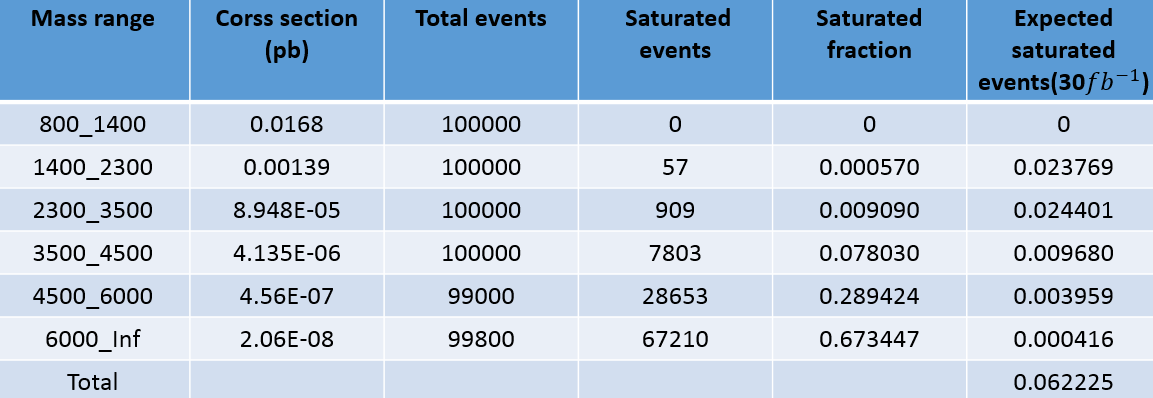
\includegraphics[width=0.9\textwidth]{chapters/Zprime/Saturation/images/FlatPt/Result/prediction.png} &
    \end{tabular}
    \caption{ The number of saturated DY events for $30~fb^{-1}$ luminosity.}
    \label{fig:Prediction_DY_s}
  \end{center}
\end{figure}

\clearpage
\subsection{Check ECAL linearity response}
\label{linearity}

Here we use MVA BDTG method training on unsaturated electron in MC and apply it to
unsaturated electron in data to check ECAL linearity response for high energy electrons.

The training target defined as:
\begin{eqnarray}
  T & = & \frac{E_{calo}}{E_{24}} \label{equ:ECAL_linearity_target}
\end{eqnarray}
where the $E_{calo}$ is the calorimeter energy of electron and $E_{24}$ is the sum energy of crystals in $5\times5$ matrix without seeded crystal.
The training input variables are listed below:
\begin{itemize}
\item $\frac{E_{left}}{E_{24}}, \frac{E_{right}}{E_{24}}, \frac{E_{top}}{E_{24}}, \frac{E_{bottom}}{E_{24}}$ : energy of the four crystals around the seed normalized to $E_{24}$
\item $\frac{E_{2\times5~ left}}{E_{24}}, \frac{E_{2\times5~ right}}{E_{24}}, \frac{E_{2\times5~top}}{E_{24}}, \frac{E_{2\times5~ bottom}}{E_{24}}$ : energy of the four $2\times5$ crystal dominoes around the seed belonging to the $5\times5$ matrix normalized to $E_{24}$
\item $\frac{E_{preShower}}{E_{24}}$ : energy measured in the PreShower normalized to $E_{24}$ (only for endcap electrons)
\item $\eta$ of the SC
\end{itemize}

The MC samples for training and testing are \texttt{ZToEE\_NNPDF30\_13TeV-powheg\_M\_400\_800 (also 800\_1400)} Moriond sample. The electrons used for training are unsaturated HEEP electrons with calorimeter energy higher than 500 GeV in barrel and 600 GeV in endcap separately. The data used for applying the MVA method are \texttt{DoubleEG\_Run2016B(C,D,E,F,G,H)\\-03Feb2017\_v*\_MINIAOD} datasets ($L \sim 35.9~fb^{-1} $).

\subsubsection{Result}
The result from MC shown in Figure \ref{fig:MC_1} is for electron energy from 500 to 700 GeV in barrel and 600 to 1000 GeV in endcap, the result in Figure \ref{fig:MC_2} is for electron energy more than 700 GeV in barrel and more than 1000 GeV in endcap. Simliarly the result from data shown in Figure \ref{fig:data_1} is for electron energy from 500 to 700 GeV in barrel and 600 to 1000 GeV in endcap, the result in Figure \ref{fig:data_2} is for electron energy more than 700 GeV in barrel and more than 1000 GeV in endcap. In order to reduce the fake electrons in data we require there are two HEEP electrons and at least one in barrel for the data event. So the result from MC in barrel is very good, for endcap the peak has around 1-2\% shift. The result from data is seems fine, the value from MAV has ~1\% lower than the reconstructed energy (calo energy).

\begin{figure}[bh]
  \begin{center}
    \begin{tabular}{cc}
      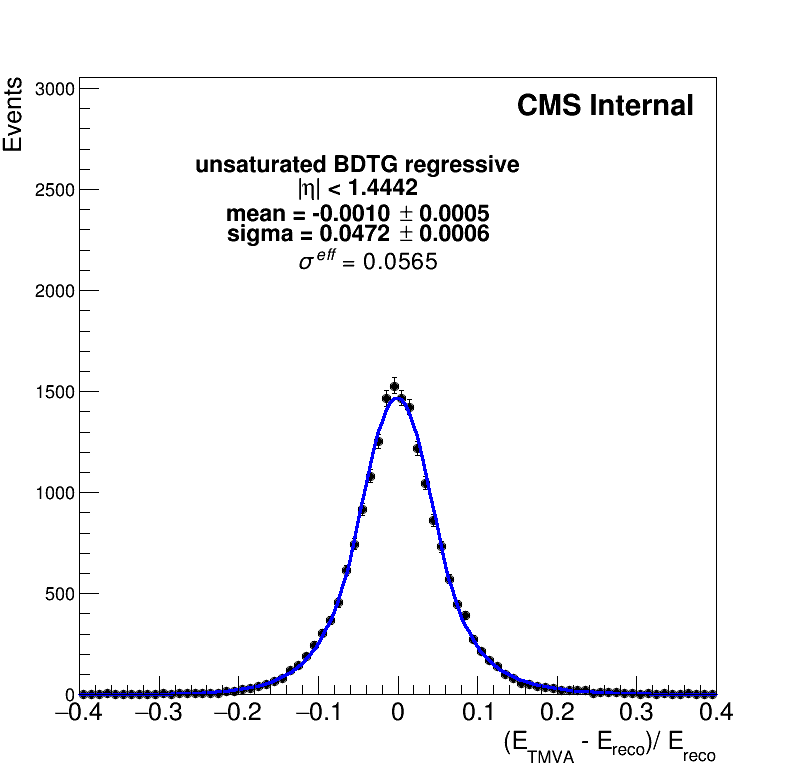
\includegraphics[width=0.45\textwidth]{chapters/Zprime/Saturation/images/ZToEE/ZToEE_B500-700_E600-1000/fit_BDTG_Barrel_Endcap_B_reg_nos.png} &
      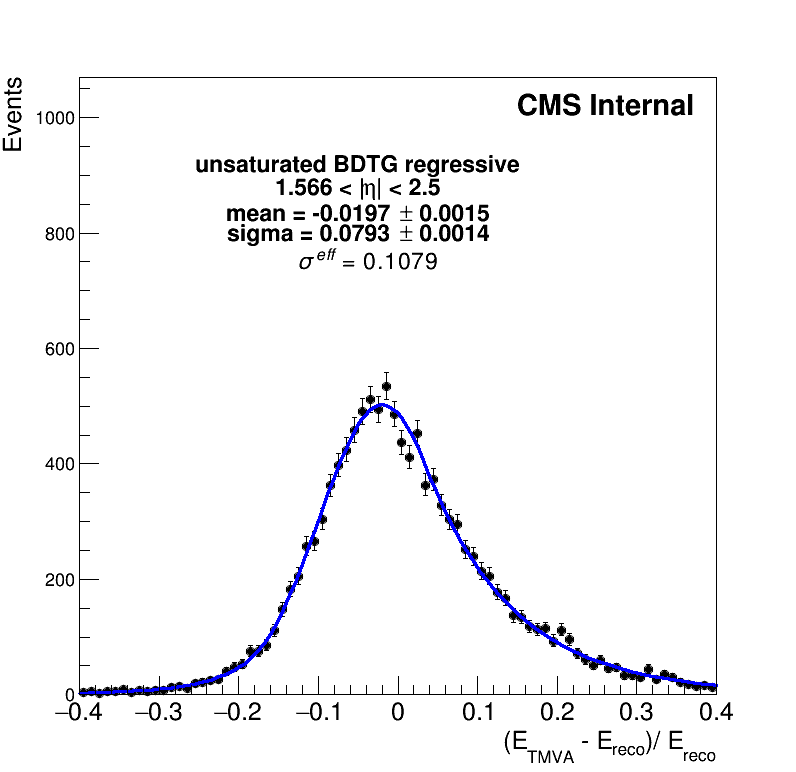
\includegraphics[width=0.45\textwidth]{chapters/Zprime/Saturation/images/ZToEE/ZToEE_B500-700_E600-1000/fit_BDTG_Barrel_Endcap_E_reg_nos.png} \\
    \end{tabular}
    \caption{ The distributions of unsaturated HEEP electrons energy from MVA minus reconstructed energy devide reconstructed energy for barrel for the reconstructed energy between 500 to 700 GeV (left) and for endcap for the reconstructed energy between 600 to 1000 GeV (right) from MC.}
    \label{fig:MC_1}
  \end{center}
\end{figure}


\begin{figure}[bh]
  \begin{center}
    \begin{tabular}{cc}
      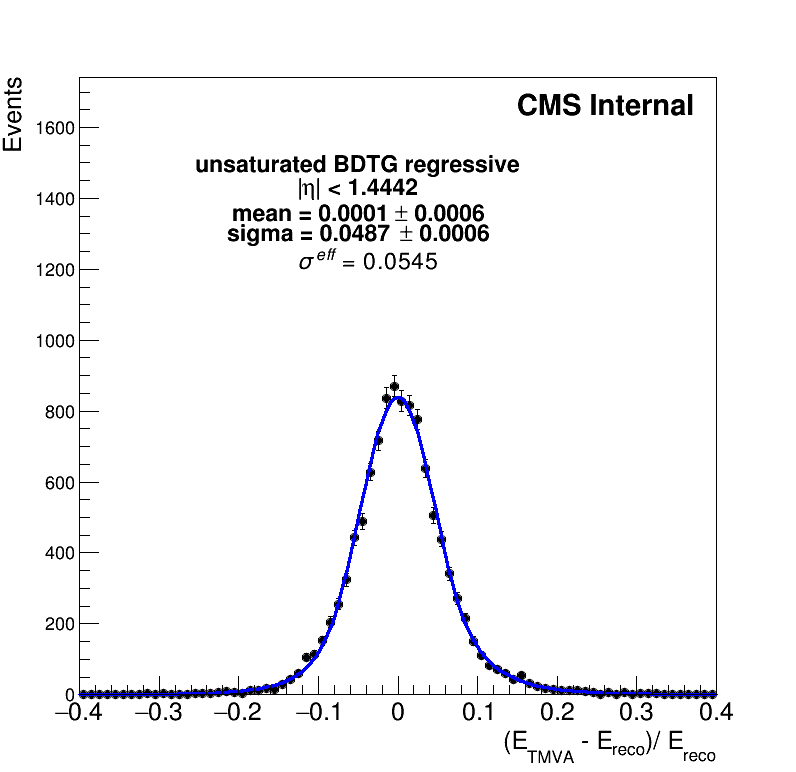
\includegraphics[width=0.45\textwidth]{chapters/Zprime/Saturation/images/ZToEE/ZToEE_B700_E1000/fit_BDTG_Barrel_Endcap_B_reg_nos.png} &
      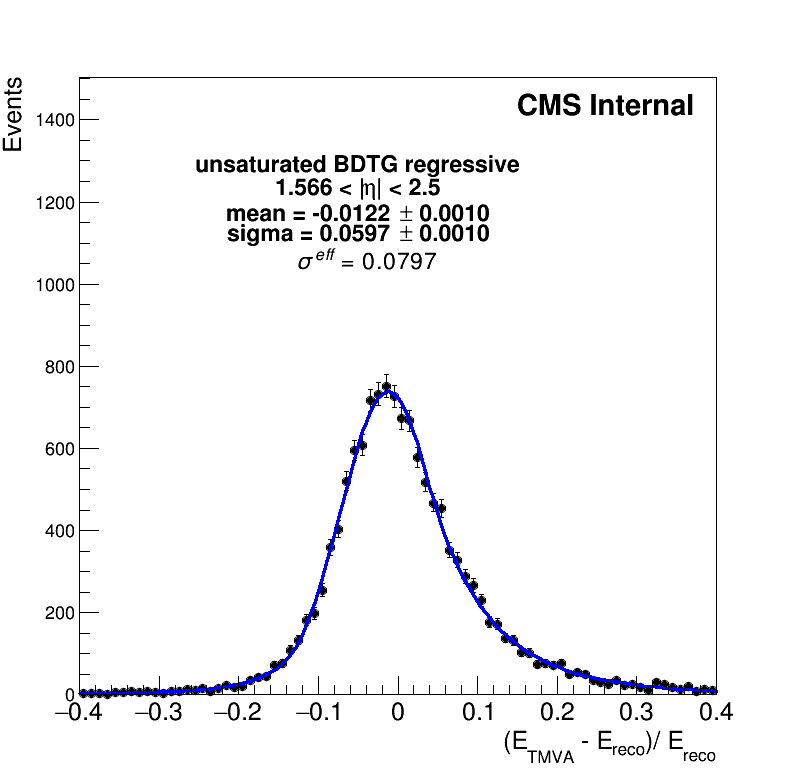
\includegraphics[width=0.45\textwidth]{chapters/Zprime/Saturation/images/ZToEE/ZToEE_B700_E1000/fit_BDTG_Barrel_Endcap_E_reg_nos.png} \\
    \end{tabular}
    \caption{ The distributions of unsaturated HEEP electrons energy from MVA minus reconstructed energy devide reconstructed energy for barrel for the reconstructed energy more than 700 GeV (left) and for endcap for the reconstructed energy more than 1000 GeV (right) from MC.}
    \label{fig:MC_2}
  \end{center}
\end{figure}


\begin{figure}[bh]
  \begin{center}
    \begin{tabular}{cc}
      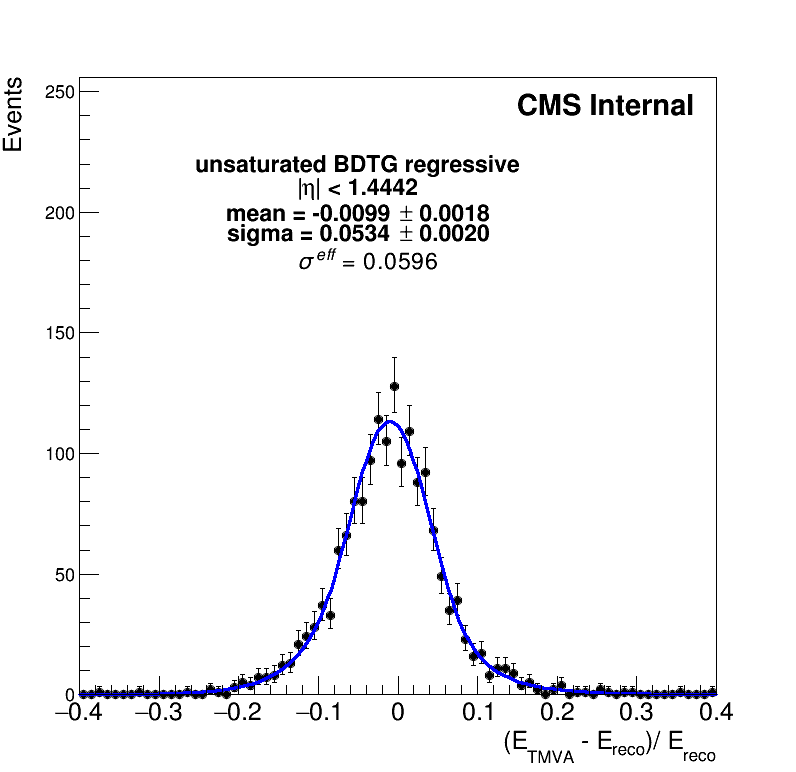
\includegraphics[width=0.45\textwidth]{chapters/Zprime/Saturation/images/ZToEE/data_B500-700_E600-1000/fit_BDTG_Barrel_Endcap_B_reg_nos.png} &
      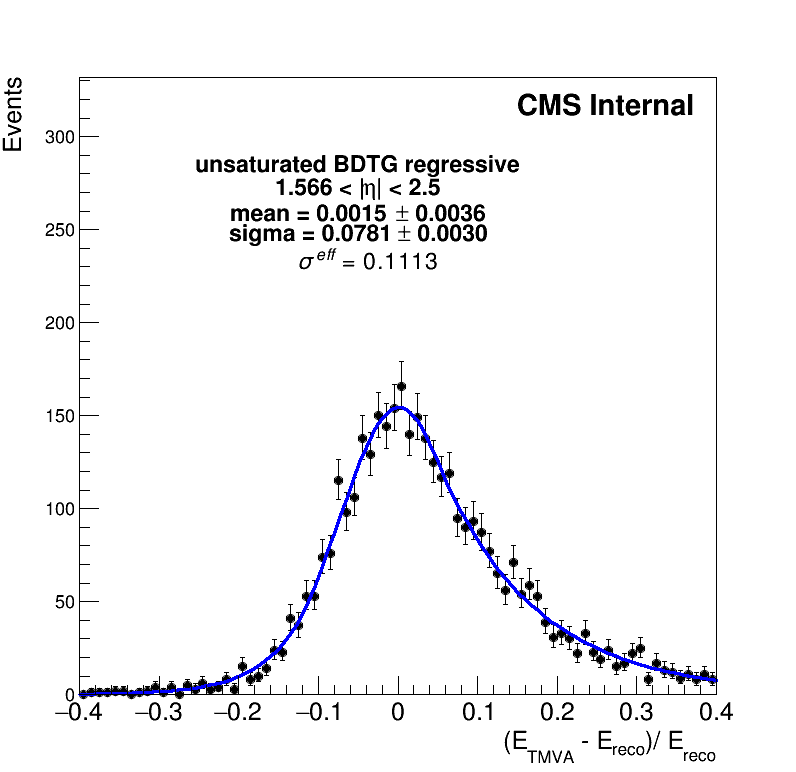
\includegraphics[width=0.45\textwidth]{chapters/Zprime/Saturation/images/ZToEE/data_B500-700_E600-1000/fit_BDTG_Barrel_Endcap_E_reg_nos.png} \\
    \end{tabular}
    \caption{ The distributions of unsaturated HEEP electrons energy from MVA minus reconstructed energy devide reconstructed energy for barrel for the reconstructed energy between 500 to 700 GeV (left) and for endcap for the reconstructed energy between 600 to 1000 GeV (right) from data.}
    \label{fig:data_1}
  \end{center}
\end{figure}


\begin{figure}[bh]
  \begin{center}
    \begin{tabular}{cc}
      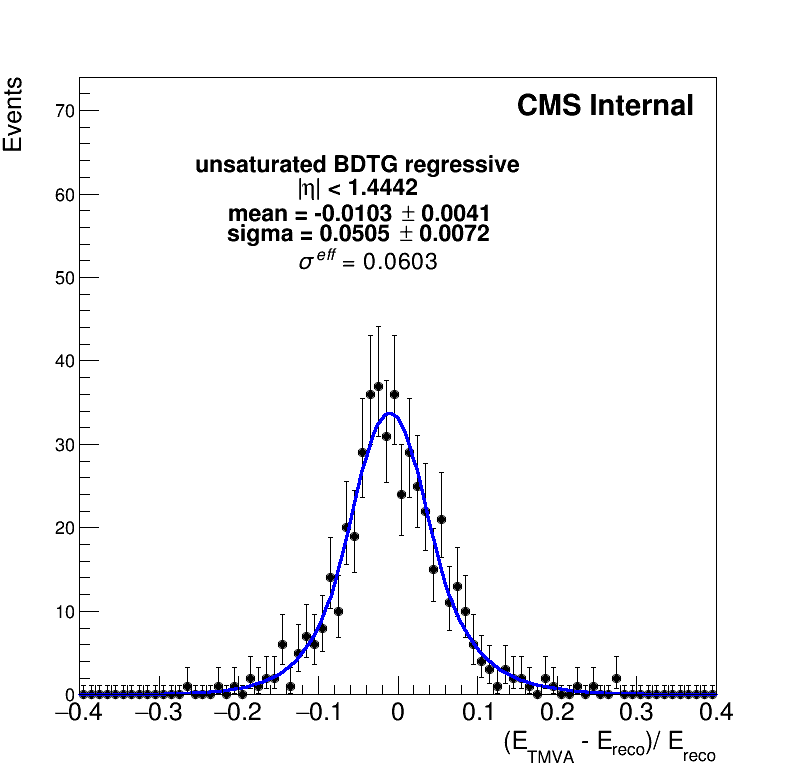
\includegraphics[width=0.45\textwidth]{chapters/Zprime/Saturation/images/ZToEE/data_B700_E1000/fit_BDTG_Barrel_Endcap_B_reg_nos.png} &
      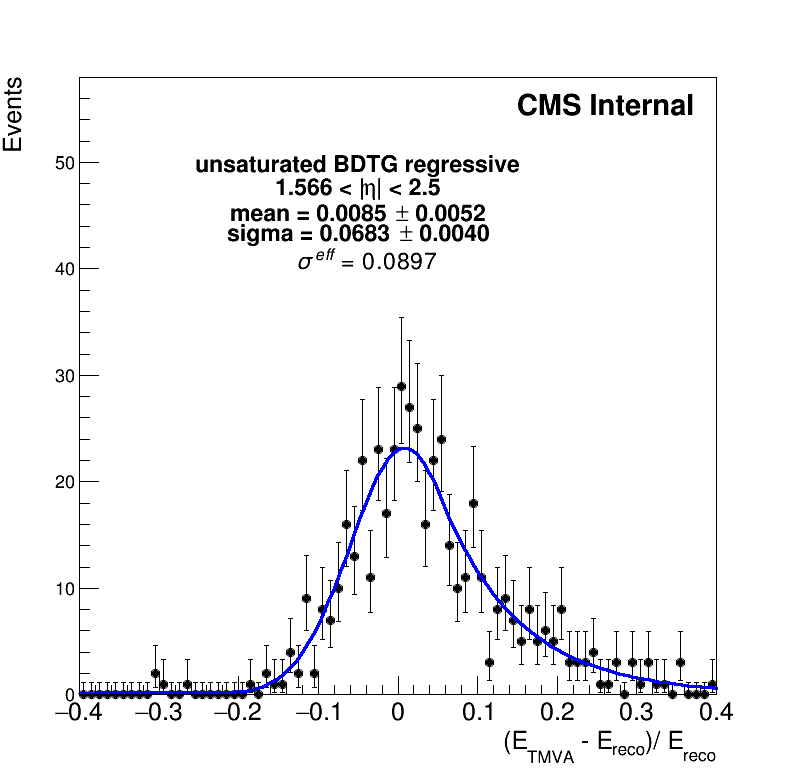
\includegraphics[width=0.45\textwidth]{chapters/Zprime/Saturation/images/ZToEE/data_B700_E1000/fit_BDTG_Barrel_Endcap_E_reg_nos.png} \\
    \end{tabular}
    \caption{ The distributions of unsaturated HEEP electrons energy from MVA minus reconstructed energy devide reconstructed energy for barrel for the reconstructed energy more than 700 GeV (left) and for endcap for the reconstructed energy more than 1000 GeV (right) from data.}
    \label{fig:data_2}
  \end{center}
\end{figure}


\clearpage
\subsection{Saturation effect to HEEP ID efficiency}
\label{HEEP_effect}
Here we use sample \texttt{/DoubleElectron\_FlatPt-300To6500/RunIISpring16DR80-\\PUFlat0to50\_80X\_mcRun2\_asymptotic\_2016\_v3-v1/AODSIM} to study the effect of saturation to HEEP ID efficiency.
The HEEP ID efficiency for saturated and unsaturated electron is shown in
Figure \ref{fig:HEEP_eff} and one can see the HEEP ID is safe for saturated
electron in endcap while for barrel it works well when the energy is lower than
around 3.2 TeV. The reason for the HEEP ID efficiency decrease quickly with energy for saturated electron in barrel is because of the showershape cut which can be seen in Figure \ref{fig:ShowerShape} and the efficiency of HEEP ID without showershape is shown in Figure \ref{fig:HEEP_noShower_eff}. The difference of the efficiency between saturated electron and unsaturated electron in Figure \ref{fig:HEEP_noShower_eff} in barrel is mainly from $\frac{H}{E}$ cut and in endcap it is mainly from EcalDriven cut.

\begin{figure}[bh]
  \begin{center}
    \begin{tabular}{cc}
      \includegraphics[width=0.45\textwidth]{chapters/Zprime/Saturation/images/FlatPt/compare_s_nos/nominal_HEEP_eff/compare_HEEP_eff_Barrel.png} &
      \includegraphics[width=0.45\textwidth]{chapters/Zprime/Saturation/images/FlatPt/compare_s_nos/nominal_HEEP_eff/compare_HEEP_eff_Endcap.png} \\
    \end{tabular}
    \caption{ The HEEP ID efficiency for saturated electron (red histogram) and unsaturated electron (blue histogram) for barrel (left) and endcap (right).}
    \label{fig:HEEP_eff}
  \end{center}
\end{figure}

\begin{figure}[bh]
  \begin{center}
    \begin{tabular}{cc}
      \includegraphics[width=0.45\textwidth]{chapters/Zprime/Saturation/images/FlatPt/compare_s_nos/compare_E15OverE55_Barrel.png} &
      \includegraphics[width=0.45\textwidth]{chapters/Zprime/Saturation/images/FlatPt/compare_s_nos/compare_E25OverE55_Barrel.png} \\
      \includegraphics[width=0.45\textwidth]{chapters/Zprime/Saturation/images/FlatPt/compare_s_nos/compare_Sieie_Endcap.png} &
    \end{tabular}
    \caption{ The distributions of the value of HEEP ID showershape variables for barrel (top) and endcap (bottom) for saturated (red histogram) and unsaturated (blue histogram) electrons.}
    \label{fig:ShowerShape}
  \end{center}
\end{figure}


\begin{figure}[bh]
  \begin{center}
    \begin{tabular}{cc}
      \includegraphics[width=0.45\textwidth]{chapters/Zprime/Saturation/images/FlatPt/compare_s_nos/noShowerShape_HEEP_eff/compare_HEEP_eff_Barrel.png} &
      \includegraphics[width=0.45\textwidth]{chapters/Zprime/Saturation/images/FlatPt/compare_s_nos/noShowerShape_HEEP_eff/compare_HEEP_eff_Endcap.png} \\
    \end{tabular}
    \caption{ The HEEP ID without showershape criteria efficiency for saturated (red histogram) and unsaturated electrons (blue histogram) for barrel (left) and endcap (right).}
    \label{fig:HEEP_noShower_eff}
  \end{center}
\end{figure}

\clearpage
\subsection{Conclusions}
In order to get the correct energy for saturated electron which has very high energy, we tried MVA method and it works well in barrel in wide energy range, for endcap there are a small bias in low erengy because of low statistics for training. Besides we also checked the ECAL linearity response in data which seems good and there are ~1\% difference between the reconstructed energy and energy from MVA. Finally we studied the effection of saturation to the HEEP ID efficiency which shows the HEEP ID still works well for saturated electron.

\clearpage
\subsection{Checking with MLP method}
\label{MLP_check}

Here we replace BDTG method with MLP method to replay the result in Figure \ref{fig:result_B_E}. The configuration of the MLP method is \texttt{factory->BookMethod( MVA::Types::kMLP, "MLP", "!H:!V:VarTransform=Norm:NeuronType=tanh:NCycles=500:HiddenLayers=N+20:\\TestRate=6:TrainingMethod=BFGS:Sampling=0.3:SamplingEpoch=0.8:\\ConvergenceImprove=1e-6:ConvergenceTests=15:!UseRegulator" )}.
From the result in Figure \ref{fig:MLP_B_E} one can see the MLP method also works but comparing with BDTG method its resolution is worse than BDTG method.
\begin{figure}[bh]
  \begin{center}
    \begin{tabular}{cc}
      \includegraphics[width=0.45\textwidth]{chapters/Zprime/Saturation/images/FlatPt/check_MLP/compare_MLP_Barrel_Endcap_enSC_B_s.png} &
      \includegraphics[width=0.45\textwidth]{chapters/Zprime/Saturation/images/FlatPt/check_MLP/compare_MLP_Barrel_Endcap_enSC_E_s.png} \\
      \includegraphics[width=0.45\textwidth]{chapters/Zprime/Saturation/images/FlatPt/check_MLP/fit_MLP_Barrel_Endcap_B_reg_s.png} &
      \includegraphics[width=0.45\textwidth]{chapters/Zprime/Saturation/images/FlatPt/check_MLP/fit_MLP_Barrel_Endcap_E_reg_s.png}
    \end{tabular}
    \caption{ The top plots are the distribution of supercluster energy minus ture energy divided by true energy for saturated electron for barrel (left) and endcap (right), the red histogram is for reconstructed supercluster enery, the blue histogram is for MVA regressive energy. The bottom plots are the fit of the blue histogram for barrel (left) and endcap (right).}
    \label{fig:MLP_B_E}
  \end{center}
\end{figure}

\clearpage
